\documentclass{article}

\usepackage{iclr2027_conference,times}
\usepackage[T1]{fontenc}
%%%%% NEW MATH DEFINITIONS %%%%%

\usepackage{amsmath,amsfonts,bm}

% Mark sections of captions for referring to divisions of figures
\newcommand{\figleft}{{\em (Left)}}
\newcommand{\figcenter}{{\em (Center)}}
\newcommand{\figright}{{\em (Right)}}
\newcommand{\figtop}{{\em (Top)}}
\newcommand{\figbottom}{{\em (Bottom)}}
\newcommand{\captiona}{{\em (a)}}
\newcommand{\captionb}{{\em (b)}}
\newcommand{\captionc}{{\em (c)}}
\newcommand{\captiond}{{\em (d)}}

% Highlight a newly defined term
\newcommand{\newterm}[1]{{\bf #1}}


% Figure reference, lower-case.
\def\figref#1{figure~\ref{#1}}
% Figure reference, capital. For start of sentence
\def\Figref#1{Figure~\ref{#1}}
\def\twofigref#1#2{figures \ref{#1} and \ref{#2}}
\def\quadfigref#1#2#3#4{figures \ref{#1}, \ref{#2}, \ref{#3} and \ref{#4}}
% Section reference, lower-case.
\def\secref#1{section~\ref{#1}}
% Section reference, capital.
\def\Secref#1{Section~\ref{#1}}
% Reference to two sections.
\def\twosecrefs#1#2{sections \ref{#1} and \ref{#2}}
% Reference to three sections.
\def\secrefs#1#2#3{sections \ref{#1}, \ref{#2} and \ref{#3}}
% Reference to an equation, lower-case.
\def\eqref#1{equation~\ref{#1}}
% Reference to an equation, upper case
\def\Eqref#1{Equation~\ref{#1}}
% A raw reference to an equation---avoid using if possible
\def\plaineqref#1{\ref{#1}}
% Reference to a chapter, lower-case.
\def\chapref#1{chapter~\ref{#1}}
% Reference to an equation, upper case.
\def\Chapref#1{Chapter~\ref{#1}}
% Reference to a range of chapters
\def\rangechapref#1#2{chapters\ref{#1}--\ref{#2}}
% Reference to an algorithm, lower-case.
\def\algref#1{algorithm~\ref{#1}}
% Reference to an algorithm, upper case.
\def\Algref#1{Algorithm~\ref{#1}}
\def\twoalgref#1#2{algorithms \ref{#1} and \ref{#2}}
\def\Twoalgref#1#2{Algorithms \ref{#1} and \ref{#2}}
% Reference to a part, lower case
\def\partref#1{part~\ref{#1}}
% Reference to a part, upper case
\def\Partref#1{Part~\ref{#1}}
\def\twopartref#1#2{parts \ref{#1} and \ref{#2}}

\def\ceil#1{\lceil #1 \rceil}
\def\floor#1{\lfloor #1 \rfloor}
\def\1{\bm{1}}
\newcommand{\train}{\mathcal{D}}
\newcommand{\valid}{\mathcal{D_{\mathrm{valid}}}}
\newcommand{\test}{\mathcal{D_{\mathrm{test}}}}

\def\eps{{\epsilon}}


% Random variables
\def\reta{{\textnormal{$\eta$}}}
\def\ra{{\textnormal{a}}}
\def\rb{{\textnormal{b}}}
\def\rc{{\textnormal{c}}}
\def\rd{{\textnormal{d}}}
\def\re{{\textnormal{e}}}
\def\rf{{\textnormal{f}}}
\def\rg{{\textnormal{g}}}
\def\rh{{\textnormal{h}}}
\def\ri{{\textnormal{i}}}
\def\rj{{\textnormal{j}}}
\def\rk{{\textnormal{k}}}
\def\rl{{\textnormal{l}}}
% rm is already a command, just don't name any random variables m
\def\rn{{\textnormal{n}}}
\def\ro{{\textnormal{o}}}
\def\rp{{\textnormal{p}}}
\def\rq{{\textnormal{q}}}
\def\rr{{\textnormal{r}}}
\def\rs{{\textnormal{s}}}
\def\rt{{\textnormal{t}}}
\def\ru{{\textnormal{u}}}
\def\rv{{\textnormal{v}}}
\def\rw{{\textnormal{w}}}
\def\rx{{\textnormal{x}}}
\def\ry{{\textnormal{y}}}
\def\rz{{\textnormal{z}}}

% Random vectors
\def\rvepsilon{{\mathbf{\epsilon}}}
\def\rvtheta{{\mathbf{\theta}}}
\def\rva{{\mathbf{a}}}
\def\rvb{{\mathbf{b}}}
\def\rvc{{\mathbf{c}}}
\def\rvd{{\mathbf{d}}}
\def\rve{{\mathbf{e}}}
\def\rvf{{\mathbf{f}}}
\def\rvg{{\mathbf{g}}}
\def\rvh{{\mathbf{h}}}
\def\rvu{{\mathbf{i}}}
\def\rvj{{\mathbf{j}}}
\def\rvk{{\mathbf{k}}}
\def\rvl{{\mathbf{l}}}
\def\rvm{{\mathbf{m}}}
\def\rvn{{\mathbf{n}}}
\def\rvo{{\mathbf{o}}}
\def\rvp{{\mathbf{p}}}
\def\rvq{{\mathbf{q}}}
\def\rvr{{\mathbf{r}}}
\def\rvs{{\mathbf{s}}}
\def\rvt{{\mathbf{t}}}
\def\rvu{{\mathbf{u}}}
\def\rvv{{\mathbf{v}}}
\def\rvw{{\mathbf{w}}}
\def\rvx{{\mathbf{x}}}
\def\rvy{{\mathbf{y}}}
\def\rvz{{\mathbf{z}}}

% Elements of random vectors
\def\erva{{\textnormal{a}}}
\def\ervb{{\textnormal{b}}}
\def\ervc{{\textnormal{c}}}
\def\ervd{{\textnormal{d}}}
\def\erve{{\textnormal{e}}}
\def\ervf{{\textnormal{f}}}
\def\ervg{{\textnormal{g}}}
\def\ervh{{\textnormal{h}}}
\def\ervi{{\textnormal{i}}}
\def\ervj{{\textnormal{j}}}
\def\ervk{{\textnormal{k}}}
\def\ervl{{\textnormal{l}}}
\def\ervm{{\textnormal{m}}}
\def\ervn{{\textnormal{n}}}
\def\ervo{{\textnormal{o}}}
\def\ervp{{\textnormal{p}}}
\def\ervq{{\textnormal{q}}}
\def\ervr{{\textnormal{r}}}
\def\ervs{{\textnormal{s}}}
\def\ervt{{\textnormal{t}}}
\def\ervu{{\textnormal{u}}}
\def\ervv{{\textnormal{v}}}
\def\ervw{{\textnormal{w}}}
\def\ervx{{\textnormal{x}}}
\def\ervy{{\textnormal{y}}}
\def\ervz{{\textnormal{z}}}

% Random matrices
\def\rmA{{\mathbf{A}}}
\def\rmB{{\mathbf{B}}}
\def\rmC{{\mathbf{C}}}
\def\rmD{{\mathbf{D}}}
\def\rmE{{\mathbf{E}}}
\def\rmF{{\mathbf{F}}}
\def\rmG{{\mathbf{G}}}
\def\rmH{{\mathbf{H}}}
\def\rmI{{\mathbf{I}}}
\def\rmJ{{\mathbf{J}}}
\def\rmK{{\mathbf{K}}}
\def\rmL{{\mathbf{L}}}
\def\rmM{{\mathbf{M}}}
\def\rmN{{\mathbf{N}}}
\def\rmO{{\mathbf{O}}}
\def\rmP{{\mathbf{P}}}
\def\rmQ{{\mathbf{Q}}}
\def\rmR{{\mathbf{R}}}
\def\rmS{{\mathbf{S}}}
\def\rmT{{\mathbf{T}}}
\def\rmU{{\mathbf{U}}}
\def\rmV{{\mathbf{V}}}
\def\rmW{{\mathbf{W}}}
\def\rmX{{\mathbf{X}}}
\def\rmY{{\mathbf{Y}}}
\def\rmZ{{\mathbf{Z}}}

% Elements of random matrices
\def\ermA{{\textnormal{A}}}
\def\ermB{{\textnormal{B}}}
\def\ermC{{\textnormal{C}}}
\def\ermD{{\textnormal{D}}}
\def\ermE{{\textnormal{E}}}
\def\ermF{{\textnormal{F}}}
\def\ermG{{\textnormal{G}}}
\def\ermH{{\textnormal{H}}}
\def\ermI{{\textnormal{I}}}
\def\ermJ{{\textnormal{J}}}
\def\ermK{{\textnormal{K}}}
\def\ermL{{\textnormal{L}}}
\def\ermM{{\textnormal{M}}}
\def\ermN{{\textnormal{N}}}
\def\ermO{{\textnormal{O}}}
\def\ermP{{\textnormal{P}}}
\def\ermQ{{\textnormal{Q}}}
\def\ermR{{\textnormal{R}}}
\def\ermS{{\textnormal{S}}}
\def\ermT{{\textnormal{T}}}
\def\ermU{{\textnormal{U}}}
\def\ermV{{\textnormal{V}}}
\def\ermW{{\textnormal{W}}}
\def\ermX{{\textnormal{X}}}
\def\ermY{{\textnormal{Y}}}
\def\ermZ{{\textnormal{Z}}}

% Vectors
\def\vzero{{\bm{0}}}
\def\vone{{\bm{1}}}
\def\vmu{{\bm{\mu}}}
\def\vtheta{{\bm{\theta}}}
\def\va{{\bm{a}}}
\def\vb{{\bm{b}}}
\def\vc{{\bm{c}}}
\def\vd{{\bm{d}}}
\def\ve{{\bm{e}}}
\def\vf{{\bm{f}}}
\def\vg{{\bm{g}}}
\def\vh{{\bm{h}}}
\def\vi{{\bm{i}}}
\def\vj{{\bm{j}}}
\def\vk{{\bm{k}}}
\def\vl{{\bm{l}}}
\def\vm{{\bm{m}}}
\def\vn{{\bm{n}}}
\def\vo{{\bm{o}}}
\def\vp{{\bm{p}}}
\def\vq{{\bm{q}}}
\def\vr{{\bm{r}}}
\def\vs{{\bm{s}}}
\def\vt{{\bm{t}}}
\def\vu{{\bm{u}}}
\def\vv{{\bm{v}}}
\def\vw{{\bm{w}}}
\def\vx{{\bm{x}}}
\def\vy{{\bm{y}}}
\def\vz{{\bm{z}}}

% Elements of vectors
\def\evalpha{{\alpha}}
\def\evbeta{{\beta}}
\def\evepsilon{{\epsilon}}
\def\evlambda{{\lambda}}
\def\evomega{{\omega}}
\def\evmu{{\mu}}
\def\evpsi{{\psi}}
\def\evsigma{{\sigma}}
\def\evtheta{{\theta}}
\def\eva{{a}}
\def\evb{{b}}
\def\evc{{c}}
\def\evd{{d}}
\def\eve{{e}}
\def\evf{{f}}
\def\evg{{g}}
\def\evh{{h}}
\def\evi{{i}}
\def\evj{{j}}
\def\evk{{k}}
\def\evl{{l}}
\def\evm{{m}}
\def\evn{{n}}
\def\evo{{o}}
\def\evp{{p}}
\def\evq{{q}}
\def\evr{{r}}
\def\evs{{s}}
\def\evt{{t}}
\def\evu{{u}}
\def\evv{{v}}
\def\evw{{w}}
\def\evx{{x}}
\def\evy{{y}}
\def\evz{{z}}

% Matrix
\def\mA{{\bm{A}}}
\def\mB{{\bm{B}}}
\def\mC{{\bm{C}}}
\def\mD{{\bm{D}}}
\def\mE{{\bm{E}}}
\def\mF{{\bm{F}}}
\def\mG{{\bm{G}}}
\def\mH{{\bm{H}}}
\def\mI{{\bm{I}}}
\def\mJ{{\bm{J}}}
\def\mK{{\bm{K}}}
\def\mL{{\bm{L}}}
\def\mM{{\bm{M}}}
\def\mN{{\bm{N}}}
\def\mO{{\bm{O}}}
\def\mP{{\bm{P}}}
\def\mQ{{\bm{Q}}}
\def\mR{{\bm{R}}}
\def\mS{{\bm{S}}}
\def\mT{{\bm{T}}}
\def\mU{{\bm{U}}}
\def\mV{{\bm{V}}}
\def\mW{{\bm{W}}}
\def\mX{{\bm{X}}}
\def\mY{{\bm{Y}}}
\def\mZ{{\bm{Z}}}
\def\mBeta{{\bm{\beta}}}
\def\mPhi{{\bm{\Phi}}}
\def\mLambda{{\bm{\Lambda}}}
\def\mSigma{{\bm{\Sigma}}}

% Tensor
\DeclareMathAlphabet{\mathsfit}{\encodingdefault}{\sfdefault}{m}{sl}
\SetMathAlphabet{\mathsfit}{bold}{\encodingdefault}{\sfdefault}{bx}{n}
\newcommand{\tens}[1]{\bm{\mathsfit{#1}}}
\def\tA{{\tens{A}}}
\def\tB{{\tens{B}}}
\def\tC{{\tens{C}}}
\def\tD{{\tens{D}}}
\def\tE{{\tens{E}}}
\def\tF{{\tens{F}}}
\def\tG{{\tens{G}}}
\def\tH{{\tens{H}}}
\def\tI{{\tens{I}}}
\def\tJ{{\tens{J}}}
\def\tK{{\tens{K}}}
\def\tL{{\tens{L}}}
\def\tM{{\tens{M}}}
\def\tN{{\tens{N}}}
\def\tO{{\tens{O}}}
\def\tP{{\tens{P}}}
\def\tQ{{\tens{Q}}}
\def\tR{{\tens{R}}}
\def\tS{{\tens{S}}}
\def\tT{{\tens{T}}}
\def\tU{{\tens{U}}}
\def\tV{{\tens{V}}}
\def\tW{{\tens{W}}}
\def\tX{{\tens{X}}}
\def\tY{{\tens{Y}}}
\def\tZ{{\tens{Z}}}


% Graph
\def\gA{{\mathcal{A}}}
\def\gB{{\mathcal{B}}}
\def\gC{{\mathcal{C}}}
\def\gD{{\mathcal{D}}}
\def\gE{{\mathcal{E}}}
\def\gF{{\mathcal{F}}}
\def\gG{{\mathcal{G}}}
\def\gH{{\mathcal{H}}}
\def\gI{{\mathcal{I}}}
\def\gJ{{\mathcal{J}}}
\def\gK{{\mathcal{K}}}
\def\gL{{\mathcal{L}}}
\def\gM{{\mathcal{M}}}
\def\gN{{\mathcal{N}}}
\def\gO{{\mathcal{O}}}
\def\gP{{\mathcal{P}}}
\def\gQ{{\mathcal{Q}}}
\def\gR{{\mathcal{R}}}
\def\gS{{\mathcal{S}}}
\def\gT{{\mathcal{T}}}
\def\gU{{\mathcal{U}}}
\def\gV{{\mathcal{V}}}
\def\gW{{\mathcal{W}}}
\def\gX{{\mathcal{X}}}
\def\gY{{\mathcal{Y}}}
\def\gZ{{\mathcal{Z}}}

% Sets
\def\sA{{\mathbb{A}}}
\def\sB{{\mathbb{B}}}
\def\sC{{\mathbb{C}}}
\def\sD{{\mathbb{D}}}
% Don't use a set called E, because this would be the same as our symbol
% for expectation.
\def\sF{{\mathbb{F}}}
\def\sG{{\mathbb{G}}}
\def\sH{{\mathbb{H}}}
\def\sI{{\mathbb{I}}}
\def\sJ{{\mathbb{J}}}
\def\sK{{\mathbb{K}}}
\def\sL{{\mathbb{L}}}
\def\sM{{\mathbb{M}}}
\def\sN{{\mathbb{N}}}
\def\sO{{\mathbb{O}}}
\def\sP{{\mathbb{P}}}
\def\sQ{{\mathbb{Q}}}
\def\sR{{\mathbb{R}}}
\def\sS{{\mathbb{S}}}
\def\sT{{\mathbb{T}}}
\def\sU{{\mathbb{U}}}
\def\sV{{\mathbb{V}}}
\def\sW{{\mathbb{W}}}
\def\sX{{\mathbb{X}}}
\def\sY{{\mathbb{Y}}}
\def\sZ{{\mathbb{Z}}}

% Entries of a matrix
\def\emLambda{{\Lambda}}
\def\emA{{A}}
\def\emB{{B}}
\def\emC{{C}}
\def\emD{{D}}
\def\emE{{E}}
\def\emF{{F}}
\def\emG{{G}}
\def\emH{{H}}
\def\emI{{I}}
\def\emJ{{J}}
\def\emK{{K}}
\def\emL{{L}}
\def\emM{{M}}
\def\emN{{N}}
\def\emO{{O}}
\def\emP{{P}}
\def\emQ{{Q}}
\def\emR{{R}}
\def\emS{{S}}
\def\emT{{T}}
\def\emU{{U}}
\def\emV{{V}}
\def\emW{{W}}
\def\emX{{X}}
\def\emY{{Y}}
\def\emZ{{Z}}
\def\emSigma{{\Sigma}}

% entries of a tensor
% Same font as tensor, without \bm wrapper
\newcommand{\etens}[1]{\mathsfit{#1}}
\def\etLambda{{\etens{\Lambda}}}
\def\etA{{\etens{A}}}
\def\etB{{\etens{B}}}
\def\etC{{\etens{C}}}
\def\etD{{\etens{D}}}
\def\etE{{\etens{E}}}
\def\etF{{\etens{F}}}
\def\etG{{\etens{G}}}
\def\etH{{\etens{H}}}
\def\etI{{\etens{I}}}
\def\etJ{{\etens{J}}}
\def\etK{{\etens{K}}}
\def\etL{{\etens{L}}}
\def\etM{{\etens{M}}}
\def\etN{{\etens{N}}}
\def\etO{{\etens{O}}}
\def\etP{{\etens{P}}}
\def\etQ{{\etens{Q}}}
\def\etR{{\etens{R}}}
\def\etS{{\etens{S}}}
\def\etT{{\etens{T}}}
\def\etU{{\etens{U}}}
\def\etV{{\etens{V}}}
\def\etW{{\etens{W}}}
\def\etX{{\etens{X}}}
\def\etY{{\etens{Y}}}
\def\etZ{{\etens{Z}}}

% The true underlying data generating distribution
\newcommand{\pdata}{p_{\rm{data}}}
% The empirical distribution defined by the training set
\newcommand{\ptrain}{\hat{p}_{\rm{data}}}
\newcommand{\Ptrain}{\hat{P}_{\rm{data}}}
% The model distribution
\newcommand{\pmodel}{p_{\rm{model}}}
\newcommand{\Pmodel}{P_{\rm{model}}}
\newcommand{\ptildemodel}{\tilde{p}_{\rm{model}}}
% Stochastic autoencoder distributions
\newcommand{\pencode}{p_{\rm{encoder}}}
\newcommand{\pdecode}{p_{\rm{decoder}}}
\newcommand{\precons}{p_{\rm{reconstruct}}}

\newcommand{\laplace}{\mathrm{Laplace}} % Laplace distribution

\newcommand{\E}{\mathbb{E}}
\newcommand{\Ls}{\mathcal{L}}
\newcommand{\R}{\mathbb{R}}
\newcommand{\emp}{\tilde{p}}
\newcommand{\lr}{\alpha}
\newcommand{\reg}{\lambda}
\newcommand{\rect}{\mathrm{rectifier}}
\newcommand{\softmax}{\mathrm{softmax}}
\newcommand{\sigmoid}{\sigma}
\newcommand{\softplus}{\zeta}
\newcommand{\KL}{D_{\mathrm{KL}}}
\newcommand{\Var}{\mathrm{Var}}
\newcommand{\standarderror}{\mathrm{SE}}
\newcommand{\Cov}{\mathrm{Cov}}
% Wolfram Mathworld says $L^2$ is for function spaces and $\ell^2$ is for vectors
% But then they seem to use $L^2$ for vectors throughout the site, and so does
% wikipedia.
\newcommand{\normlzero}{L^0}
\newcommand{\normlone}{L^1}
\newcommand{\normltwo}{L^2}
\newcommand{\normlp}{L^p}
\newcommand{\normmax}{L^\infty}

\newcommand{\parents}{Pa} % See usage in notation.tex. Chosen to match Daphne's book.

\DeclareMathOperator*{\argmax}{arg\,max}
\DeclareMathOperator*{\argmin}{arg\,min}

\DeclareMathOperator{\sign}{sign}
\DeclareMathOperator{\Tr}{Tr}
\let\ab\allowbreak

\usepackage{amsmath,amssymb,amsfonts}
\usepackage{booktabs}
\usepackage{graphicx}
\usepackage{multirow}
\usepackage{array}
\usepackage{url}
\usepackage{hyperref}
\hypersetup{colorlinks=false,citebordercolor={0 1 0}}
\pdfsuppresswarningpagegroup=1

\providecommand{\R}{\mathbb{R}}
\providecommand{\Sph}{\mathbb{S}}
\providecommand{\Tangent}{\mathcal{T}}
\providecommand{\M}{\mathcal{M}}
\providecommand{\ReLU}{\operatorname{ReLU}}
\providecommand{\rank}{\operatorname{rank}}
\providecommand{\prox}{\operatorname{prox}}
\providecommand{\LN}{\operatorname{LN}}
\providecommand{\vecop}{\operatorname{vec}}
\providecommand{\softmax}{\operatorname{softmax}}
\providecommand{\argmax}{\operatorname*{arg\,max}}
\providecommand{\argmin}{\operatorname*{arg\,min}}

\title{Reliability-Conditioned Product-Tangent Learning for Degraded Acoustics}
\author{Anonymous Authors}

\begin{document}
\maketitle

\begin{abstract}
Synchronized acoustic descriptors offer complementary views of one signal, but they do not fail uniformly: impulsive, co-channel, and additive interference perturb their coordinates, norms, and temporal structure in different ways. A corrupted high-energy descriptor can therefore dominate Euclidean relation learning even when another domain retains useful evidence. We study this failure as reliability-conditioned geometric representation learning. The proposed RMAL-CRNN first estimates coordinate reliability, then applies descriptor-specific spherical tangent projections. Head-specific tangent-metric attention learns cross-domain relations after this correction, and a factorized nonnegative sparse affinity refines the fused sequence over time. Controlled simulations show how these stages respond to individual and compound degradations. Across a public ten-class UAV benchmark and an independent eight-class Glasgow/ACSAC~2022 acoustic-identity release, the complete model reaches $86.30\%$ and $93.88\%$ on the ten-class benchmark at $-5$ and $0$ dB, and $81.18\%$ at $0$ dB on Glasgow versus $74.28\%$ for CRNN. Multi-seed ablations favor the complete path. These results establish a consistent advantage for reliability-before-relation learning across the evaluated descriptors, public benchmarks, and degradation conditions.
\end{abstract}

\section{Introduction}

Acoustic observations are often represented by several synchronized descriptors rather than one homogeneous vector. Time-, frequency-, cepstral-, and time--frequency-domain transforms expose different signal structure, and modern audio networks can learn rich temporal or spectrotemporal representations \citep{cakir2017crnn,kong2020panns,gong2021ast}. Complementarity alone is not enough under corruption. An impulse may disrupt energy-localized coordinates, co-channel interference may inflate a domain norm, and diffuse noise may erase temporal structure. Since the domains differ in scale, interpretation, and sensitivity, the same perturbation does not reduce their reliability equally. The learning problem is thus not merely how to fuse several views, but how to keep a damaged view from determining the relations among all of them.

Recent acoustic models improve representation capacity through pretraining, attention, spatial reconstruction, relation-aware scene modeling, and disentanglement across cities or devices \citep{hou2024cooperative,yang2024spatial,tan2024disentanglement}. These advances address important variability, yet synchronized handcrafted descriptors are usually treated as Euclidean channels or tokens. Under unequal corruption, an expressive fusion operator can still compare domains before it knows which coordinates are trustworthy. Fixed concatenation has the same weakness in a simpler form: high magnitude is indistinguishable from high reliability. We ask a narrower question. Can reliability be estimated before relation learning while each descriptor retains a domain-specific geometry?

Several mature ideas inform the answer, but none is the claim of this paper by itself. Robust Student-$t$ statistics attenuate large standardized residuals \citep{lange1989student}; manifold and subspace methods preserve non-Euclidean or self-expressive structure \citep{roweis2000lle,tenenbaum2000isomap,vidal2011subspace}; geometric deep learning embeds such structure in trainable models \citep{bronstein2017gdl,chakraborty2022manifoldnet}; and attention or differentiable affinity layers learn relations end to end \citep{vaswani2017attention,velickovic2018gat,ji2017dsc}. What remains unresolved here is their ordering under compound acoustic degradation. Reliability must precede geometric comparison, the domains must not be collapsed into one tangent plane, and temporal refinement must not obscure whether the cross-domain relation itself was well formed.

We instantiate this ordering in a robust manifold-attention low-rank convolutional recurrent network (RMAL-CRNN). Figure~\ref{fig:framework} previews the path. Our contribution is threefold:
\begin{itemize}
  \item We formulate compound-corruption learning as reliability-conditioned relation estimation across synchronized, noncommensurate descriptor domains. The formulation distinguishes descriptor identity from modality or dataset domain and makes unequal reliability an explicit learning variable.
  \item We construct a product of learned spherical tangent spaces, then evaluate cross-domain relations with head-specific tangent-metric attention. The projection follows the corresponding spherical log-map direction blockwise; the attention distribution has a finite-bandwidth concentration envelope; and the subsequent raw temporal affinity has an explicit rank budget with nonnegative proximal thresholding.
  \item We align evidence with the proposed order without conflating protocols. Controlled individual and compound degradations probe stage-specific behavior and representation geometry; a separate SNR-conditioned public-data study reports multi-seed comparisons, structural ablations, confidence intervals, effect sizes, and Holm-corrected paired tests. All conclusions are restricted to the evaluated data and corruption ranges.
\end{itemize}

\section{Related Work}

\paragraph{Acoustic representation learning.}
Convolutional-recurrent networks, large-scale pretrained audio networks, and spectrogram transformers learn temporal or time--frequency representations directly \citep{cakir2017crnn,kong2020panns,gong2021ast}. More recent work models cooperative scene--event relations, reconstructs spatial channels without labels, or disentangles city and device factors \citep{hou2024cooperative,yang2024spatial,tan2024disentanglement}. We study synchronized fixed descriptors whose physical roles and corruption sensitivities differ, and organize them through a reliability-conditioned geometric representation path. This representation provides a foundation for future integration with learned acoustic front ends.

\paragraph{Geometry and robust subspaces.}
Local manifold learning and subspace clustering established complementary ways to preserve neighborhood or self-expression structure \citep{roweis2000lle,tenenbaum2000isomap,elhamifar2013ssc,liu2013lrr}. Geometric deep networks extend learning beyond Euclidean inputs \citep{bronstein2017gdl,chakraborty2022manifoldnet}. Building on these foundations, our construction uses robust coordinate weights before mapping each descriptor to a separate learned spherical tangent block, so a common ambient dimension preserves domain identity.

\paragraph{Structured attention and affinity.}
Standard attention learns token interactions from queries and keys \citep{vaswani2017attention}; graph attention and deep self-expression add structural constraints \citep{velickovic2018gat,ji2017dsc}. Squared-distance attention also has known stability distinctions from unconstrained dot-product attention \citep{kim2021lipschitz}. Here the queries and keys are projected onto learned head-specific tangent planes and compared by squared Euclidean distance in those planes. A separate factorized, nonnegative sparse relation then operates over time. This separation lets the controlled experiments ask whether cross-domain and temporal relations respond to different failure modes.

\section{Reliability-Conditioned Product-Tangent Learning}

\subsection{Problem Setup}
Let $\mathbf r_t\in\R^L$ denote the $t$-th acoustic frame and let $K$ fixed transforms produce synchronized descriptor blocks
\begin{equation}
\mathbf x_t^{(k)}=\mathcal F_k(\mathbf r_t)\in\R^{d_k},\qquad
\mathbf x_t=\operatorname{concat}_{k=1}^{K}\mathbf x_t^{(k)}.
\label{eq:domain-feature}
\end{equation}
The full observation is $\mathbf X=[\mathbf x_1^\top;\ldots;\mathbf x_T^\top]\in\R^{T\times D_\Sigma}$, where $T$ is the frame count, $D_\Sigma=\sum_k d_k$, and $y$ is the class label. These blocks are transforms of the same frame, not independent modalities or dataset domains. The implemented model uses $K=6$ equal blocks with $d_k=d=32$. We seek a classifier $p(y\mid\mathbf X)$ that remains useful when a corruption changes block statistics and coordinate reliability unequally.

For a unit base point $\mathbf p_k\in\Sph^{d-1}$, define the spherical tangent space
\begin{equation}
\Tangent_{\mathbf p_k}\Sph^{d-1}
=\{\mathbf u\in\R^d:\mathbf p_k^\top\mathbf u=0\}.
\label{eq:tangent-space}
\end{equation}
The GST projected components occupy the product
\begin{equation}
\M=\prod_{k=1}^{K}\Tangent_{\mathbf p_k}\Sph^{d-1},
\qquad \dim(\M)=K(d-1).
\label{eq:product-space}
\end{equation}
Separate base points preserve descriptor-specific directions in a common ambient dimension. Subsequent learned biases translate the projected components into affine tangent spaces.

\subsection{Ordered Representation Path}
Figure~\ref{fig:framework} shows the complete path. Reliability weighting is applied before any cross-domain comparison. Each corrected block is projected to a learned spherical tangent space; tangent-metric attention then estimates relations among the $K$ domains. Only after this cross-domain fusion do we construct a compact sparse affinity over the $T$ frames. The ordering is not cosmetic: the controlled experiments separately probe coordinate outliers, input-scale sensitivity, temporal noise, and their compound action.

\begin{figure}[t]
  \centering
  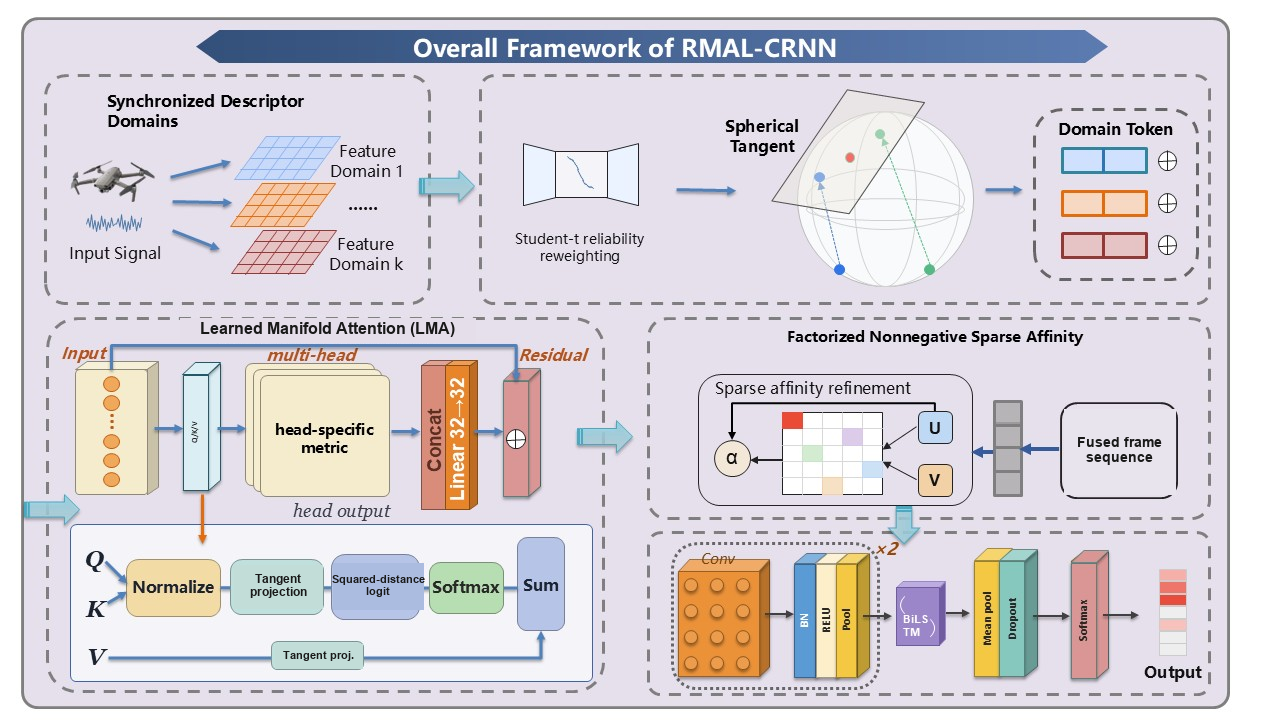
\includegraphics[width=\linewidth]{figures/fig1.png}
  \caption{Ordered RMAL-CRNN path. Coordinate reliability precedes domain-specific tangent projection and cross-domain relation learning. The fused frame sequence then parameterizes learned factors for temporal affinity refinement.}
  \label{fig:framework}
\end{figure}

\subsection{Geometric Student-t Tangent-Subspace Projection (GST)}
Heavy-tailed deviations motivate a Student-$t$-shaped reliability score \citep{lange1989student}. For domain $k$, learn a center $\boldsymbol\mu_k\in\R^d$, scale parameters $\boldsymbol\alpha_k\in\R^d$, and log-inverse degrees of freedom $\boldsymbol\eta_k\in\R^d$. Coordinatewise, $\boldsymbol\sigma_k=\max(\exp(\boldsymbol\alpha_k),\epsilon\mathbf1)$ and $\nu_{k,j}=1/\operatorname{clip}(e^{\eta_{k,j}},10^{-4},1)$. With stabilizer $\epsilon>0$, all-ones vector $\mathbf1$, elementwise division $\oslash$, and Hadamard product $\odot$, the standardized residual $\boldsymbol\rho_t^{(k)}$, reliability vector $\mathbf g_t^{(k)}$, and corrected block $\widehat{\mathbf x}_t^{(k)}$ are
\begin{align}
\boldsymbol\rho_t^{(k)}
&=(\mathbf x_t^{(k)}-\boldsymbol\mu_k)
\oslash\boldsymbol\sigma_k,\nonumber\\
\mathbf g_t^{(k)}
&=(\boldsymbol\nu_k+\mathbf1)\oslash
\left(\boldsymbol\nu_k+\boldsymbol\rho_t^{(k)}\odot\boldsymbol\rho_t^{(k)}\right),\nonumber\\
\widehat{\mathbf x}_t^{(k)}&=\mathbf g_t^{(k)}\odot\mathbf x_t^{(k)}.
\label{eq:gst-gate}
\end{align}
Here $\boldsymbol\nu_k=(\nu_{k,1},\ldots,\nu_{k,d})^\top$ and $\epsilon=10^{-6}$. Each entry satisfies $0<g_{t,j}^{(k)}\leq1+1/\nu_{k,j}$: coordinates near the learned center retain or mildly increase their weight, while large standardized residuals are attenuated.

For the equal-dimensional blocks used here, the corrected block is projected directly by $\Pi_{\mathbf p_k}$:
\begin{align}
\mathbf h_t^{(k)}&=\widehat{\mathbf x}_t^{(k)},
&\mathbf h_t^{(k)}&\in\R^d,
\label{eq:domain-alignment}\\
\mathbf p_k&=\frac{\overline{\mathbf p}_k}{\max(\|\overline{\mathbf p}_k\|_2,\epsilon)},
&\Pi_{\mathbf p_k}&=\mathbf I_d-\mathbf p_k\mathbf p_k^\top,
\label{eq:domain-basepoint}\\
\mathbf u_t^{(k)}&=\Pi_{\mathbf p_k}\mathbf h_t^{(k)}.
\label{eq:tangent-projection}
\end{align}
The projected component $\mathbf u_t^{(k)}$ lies in the tangent plane. The implementation then normalizes it and adds an unconstrained learned domain bias $\mathbf b_k$:
\begin{equation}
\mathbf z_t^{(k)}
=\sqrt d\,\frac{\mathbf u_t^{(k)}}{\max(\|\mathbf u_t^{(k)}\|_2,\epsilon)}
+\mathbf b_k.
\label{eq:token}
\end{equation}
Stacking gives $\mathbf Z_t=[\mathbf z_t^{(1)},\ldots,\mathbf z_t^{(K)}]^\top\in\R^{K\times d}$. Appendix~\ref{app:blockwise} proves blockwise directional agreement with the spherical logarithmic map on the unit-normalization branch $\|\overline{\mathbf p}_k\|_2\geq\epsilon$. The normalized component lies in its tangent space; adding $\mathbf b_k$ yields an affine tangent token.

\subsection{Learned Manifold Attention (LMA) with Tangent Metrics}
We add an unconstrained learned domain embedding $\mathbf e_k$ to retain source identity, $\widetilde{\mathbf z}_t^{(k)}=\mathbf z_t^{(k)}+\mathbf e_k$. For head $h\in\{1,\ldots,N_h\}$, let $d_h=d/N_h$, normalize a learned base point $\mathbf p_h$ with the same $\epsilon$ safeguard, and set $\Pi_{\mathbf p_h}=\mathbf I-\mathbf p_h\mathbf p_h^\top$. The matrices $\mathbf W_q^h$, $\mathbf W_k^h$, and $\mathbf W_v^h$ are learned query, key, and value maps. Queries and keys are normalized before projection; values are projected into the same head tangent plane. The tangent interpretation uses unit base points; the residual and LayerNorm operate in the ambient feature space:
\begin{equation}
\begin{aligned}
\overline{\mathbf q}_i^h&=\frac{\mathbf W_q^h\widetilde{\mathbf z}_t^{(i)}}
{\max(\|\mathbf W_q^h\widetilde{\mathbf z}_t^{(i)}\|_2,\epsilon)},
&\mathbf q_i^h&=\Pi_{\mathbf p_h}\overline{\mathbf q}_i^h,\\
\overline{\mathbf k}_j^h&=\frac{\mathbf W_k^h\widetilde{\mathbf z}_t^{(j)}}
{\max(\|\mathbf W_k^h\widetilde{\mathbf z}_t^{(j)}\|_2,\epsilon)},
&\mathbf k_j^h&=\Pi_{\mathbf p_h}\overline{\mathbf k}_j^h,\\
\mathbf v_j^h&=\Pi_{\mathbf p_h}\mathbf W_v^h\widetilde{\mathbf z}_t^{(j)}.
\end{aligned}
\label{eq:qkv}
\end{equation}
Instead of a dot product, the logit is the negative squared distance induced by the flat metric of the learned tangent plane:
\begin{align}
\ell_{ij}^h&=-\gamma_h\|\mathbf q_i^h-\mathbf k_j^h\|_2^2,
&\gamma_h&=\exp(\overline\gamma_h)>0,
\label{eq:attention-logit}\\
a_{ij}^h&=\frac{\exp(\ell_{ij}^h)}{\sum_{m=1}^{K}\exp(\ell_{im}^h)}.
\label{eq:attention-weight}
\end{align}
With output map $\mathbf W_o$ and LayerNorm operator $\LN$, the attended tokens $\mathbf y_{t,i}$ are
\begin{equation}
\mathbf y_{t,i}=\LN\!\left(\widetilde{\mathbf z}_t^{(i)}+
\mathbf W_o\operatorname{concat}_{h=1}^{N_h}
\sum_{j=1}^{K}a_{ij}^h\mathbf v_j^h\right).
\label{eq:attention-output}
\end{equation}

Normalization and orthogonal projection imply 
$\|\mathbf q_i^h-\mathbf k_j^h\|_2^2\leq4$. Hence the logits are bounded in $[-4\gamma_h,0]$, and Appendix~\ref{app:attention-proof} gives a finite-bandwidth upper bound on the largest attention weight and a corresponding entropy lower bound. The head base point removes one learned direction from each preprojected difference:
\begin{equation}
\|\Pi_{\mathbf p_h}(\overline{\mathbf q}-\overline{\mathbf k})\|_2^2
=\|\overline{\mathbf q}-\overline{\mathbf k}\|_2^2
-\big((\overline{\mathbf q}-\overline{\mathbf k})^\top\mathbf p_h\big)^2.
\label{eq:head-geometry}
\end{equation}
Different heads therefore learn complementary rank-$(d_h-1)$ metrics. The distinction from standard attention \citep{vaswani2017attention} is the learned tangent projector and its squared-distance kernel in that plane, not attention as a general operation.

\subsection{Factorized Nonnegative Sparse Affinity Refinement (FNSAR)}
After concatenating the $K$ attended tokens, a QR-initialized learned linear map yields one frame vector $\mathbf f_t\in\R^{d_f}$, and $\mathbf F=[\mathbf f_1,\ldots,\mathbf f_T]^\top$. Learned factor maps $\mathbf W_u,\mathbf W_v\in\R^{r_\ell\times d_f}$ construct a directed temporal relation with rank budget $r_\ell$:
\begin{equation}
\begin{alignedat}{2}
\mathbf U&=\mathbf F\mathbf W_u^\top &\quad&\in\R^{T\times r_\ell},\\
\mathbf V&=\mathbf F\mathbf W_v^\top &&\in\R^{T\times r_\ell},\\
\mathbf C_{\mathrm{raw}}&=r_\ell^{-1/2}\mathbf U\mathbf V^\top &&\in\R^{T\times T},\\
\mathbf C&=\ReLU\!\left(\mathbf C_{\mathrm{raw}}-\vartheta\mathbf1\mathbf1^\top\right),
&&\vartheta=\exp(\overline\vartheta)>0.
\end{alignedat}
\label{eq:fnsar-affinity}
\end{equation}
Here $\mathbf1\mathbf1^\top\in\R^{T\times T}$, $\ReLU$ acts entrywise, and the learned positive threshold is $\vartheta$. The raw affinity satisfies $\rank(\mathbf C_{\mathrm{raw}})\leq r_\ell$. Entrywise thresholding is the proximal map of a nonnegative $\ell_1$ penalty: at fixed $\mathbf C_{\mathrm{raw}}$, increasing $\vartheta$ removes support. The rank budget applies to the raw factorized relation; thresholding controls the support of $\mathbf C$. The refined output retains a direct residual path, with logistic sigmoid $\sigma$ setting the learned mixing coefficient $\zeta$:
\begin{equation}
\mathbf f_t^{\mathrm{out}}
=(1-\zeta)\mathbf f_t+
\zeta\,\LN\!\left(\sum_{s=1}^{T}C_{ts}\mathbf f_s\right),
\qquad \zeta=\sigma(\overline\zeta)\in(0,1).
\label{eq:fnsar-output}
\end{equation}
Appendix~\ref{app:affinity} proves the rank, proximal-support, and LayerNorm-residual bounds. This construction is related to differentiable self-expression \citep{elhamifar2013ssc,liu2013lrr,ji2017dsc}, but operates on the already fused temporal sequence and explicitly enforces nonnegative sparse support.

\subsection{Training and Cost}
The output sequence is classified by a CRNN. With label-smoothed cross-entropy $\mathcal L_{\mathrm{cls}}$, factor and sparsity weights $\lambda_{\mathrm{fac}}=\lambda_{\mathrm{sps}}=10^{-3}$, and elementwise squaring, training minimizes
\begin{equation}
\mathcal L=\mathcal L_{\mathrm{cls}}
+\frac{\lambda_{\mathrm{fac}}}{2}
\left[\operatorname{mean}(\mathbf U\odot\mathbf U)+\operatorname{mean}(\mathbf V\odot\mathbf V)\right]
+\lambda_{\mathrm{sps}}\operatorname{mean}(|\mathbf C|).
\label{eq:objective}
\end{equation}
Here $\operatorname{mean}$ averages every entry, including the minibatch dimension, and the cross-entropy uses smoothing $0.1$. The cross-domain attention costs $O(TK^2d)$ after linear projections. Temporal affinity formation and aggregation cost $O(T^2r_\ell)$ and $O(T^2d_f)$; the method remains quadratic in sequence length but avoids iterative singular-value decomposition. Appendix~\ref{app:implementation} records the complete configuration and hyperparameter study.

\section{Experiments}

The experiments address three questions. \textbf{Q1:} Do the stages respond to the failure modes they were designed for? \textbf{Q2:} Does the complete path improve classification across the evaluated SNRs? \textbf{Q3:} Are its gains consistent across matched random seeds and structural removals? Full signal-generation controls, feature definitions, and implementation settings appear in Appendix~\ref{app:experimental-details}.

\subsection{Protocol}
The controlled study combines a class-dependent rotating-source model with coherent paths, modulation, turbulence, sparse impulses, co-channel interference, and diffuse Gaussian noise. The latter three are varied independently through impulse intensity $\kappa$, signal-to-interference ratio (SIR), and SNR, then superimposed for the compound condition. Six synchronized 32-dimensional descriptor domains are extracted: HHT, LOFAR, FFT, WPT, HHSA, and MFCC. These controls define the normalized simulation conditions used in the mechanism study.

The public-data study combines two complementary benchmarks. The Kielce benchmark uses ten UAV-model classes from the public release \href{https://zenodo.org/records/15190811}{Zenodo record 15190811} \citep{miesikowska2023uavdataset}: five quadrotor (X4) models and five hexarotor (X6) models, listed in Table~\ref{tab:kielce-models}. Glasgow/ACSAC~2022 \citep{diao2022drone} contributes eight acoustic-identity groups from DJI Mini~2 recordings (44.1-kHz, 16-bit, single-channel WAV) captured at 1~m and 5~m, including distinct propeller configurations. Released SNR conditions are evaluated directly after the common six-domain feature extraction. Each benchmark uses a fixed split, shared optimization settings, and repeated random-seed runs; results are mean accuracy with sample standard deviation. Appendix~\ref{app:implementation} records the selected hyperparameters and model compositions.

The controlled study and public benchmarks provide complementary evidence. Q1 uses the full simulator to isolate stage responses to individual and compound degradations. Q2--Q3 evaluate low-SNR classification on the released datasets, while the simulator clarifies how each proposed stage responds to targeted degradation mechanisms.

\subsection{Q1: Controlled Mechanism Tests}
Figure~\ref{fig:mechanisms} places direct diagnostics from all three stages on a common visual baseline. Under impulses, GST changes descriptor reliability selectively rather than scaling every domain together. Under co-channel interference, the tangent-metric LMA logits remain inside their finite admissible interval, whereas the unnormalized dot-product control spans a much wider range. Under additive noise, FNSAR preserves a larger top-$8$ spectral-energy fraction than the raw representation at low SNR. Full descriptor-sensitivity, fusion-fidelity, peak-attention, affinity, and representation-drift plots appear in Appendix~\ref{app:mechanism-panels}. These diagnostics isolate stage behavior and complement the end-to-end classification results.

\begin{figure*}[t]
  \centering
  \begin{minipage}[t]{0.318\textwidth}
    \centering
    \fontsize{7.5}{8.5}\selectfont (a)\\[-0.45em]
        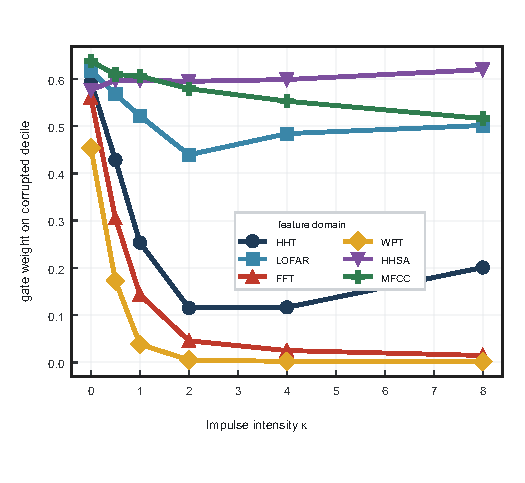
\includegraphics[width=\linewidth]{figures/fig2a.pdf}
  \end{minipage}\hfill%
  \begin{minipage}[t]{0.318\textwidth}
    \centering
    \fontsize{7.5}{8.5}\selectfont (b)\\[-0.45em]
        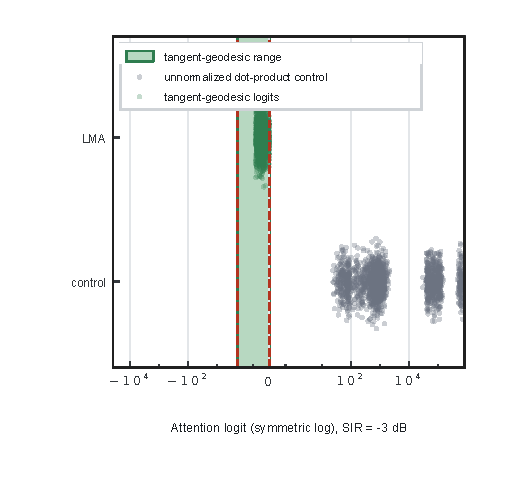
\includegraphics[width=\linewidth]{figures/fig2b.pdf}
  \end{minipage}\hfill%
  \begin{minipage}[t]{0.318\textwidth}
    \centering
    \fontsize{7.5}{8.5}\selectfont (c)\\[-0.45em]
        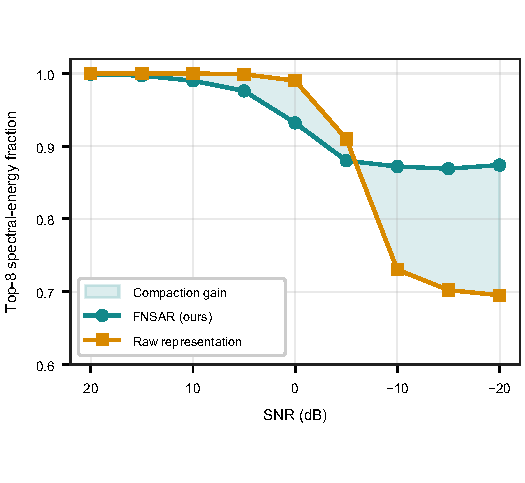
\includegraphics[width=\linewidth]{figures/fig2c.pdf}
  \end{minipage}
  \caption{Controlled mechanism diagnostics assembled from separately extracted vector panels. (a) GST reliability across descriptor domains versus impulse intensity. (b) Tangent-metric LMA logits and an unnormalized dot-product control at SIR $=-3$ dB. (c) Top-$8$ spectral-energy fraction before and after FNSAR.}
  \label{fig:mechanisms}
\end{figure*}

The compound condition is the harder mechanism test because all three failures act simultaneously. Figure~\ref{fig:compound-geometry} shows two complementary UMAP diagnostics from the controlled study. At the sample level, compound degradation disperses and overlaps class embeddings; after the complete model, the plotted clusters become more compact and separated. At the descriptor level, corruption disturbs the relative organization of the six domains, while reliability weighting and tangent projection tighten the domain clusters. Together, the two views show how the proposed reliability-conditioned geometry organizes both class-level and descriptor-level representations under compound degradation.

\begin{figure}[t]
  \centering
  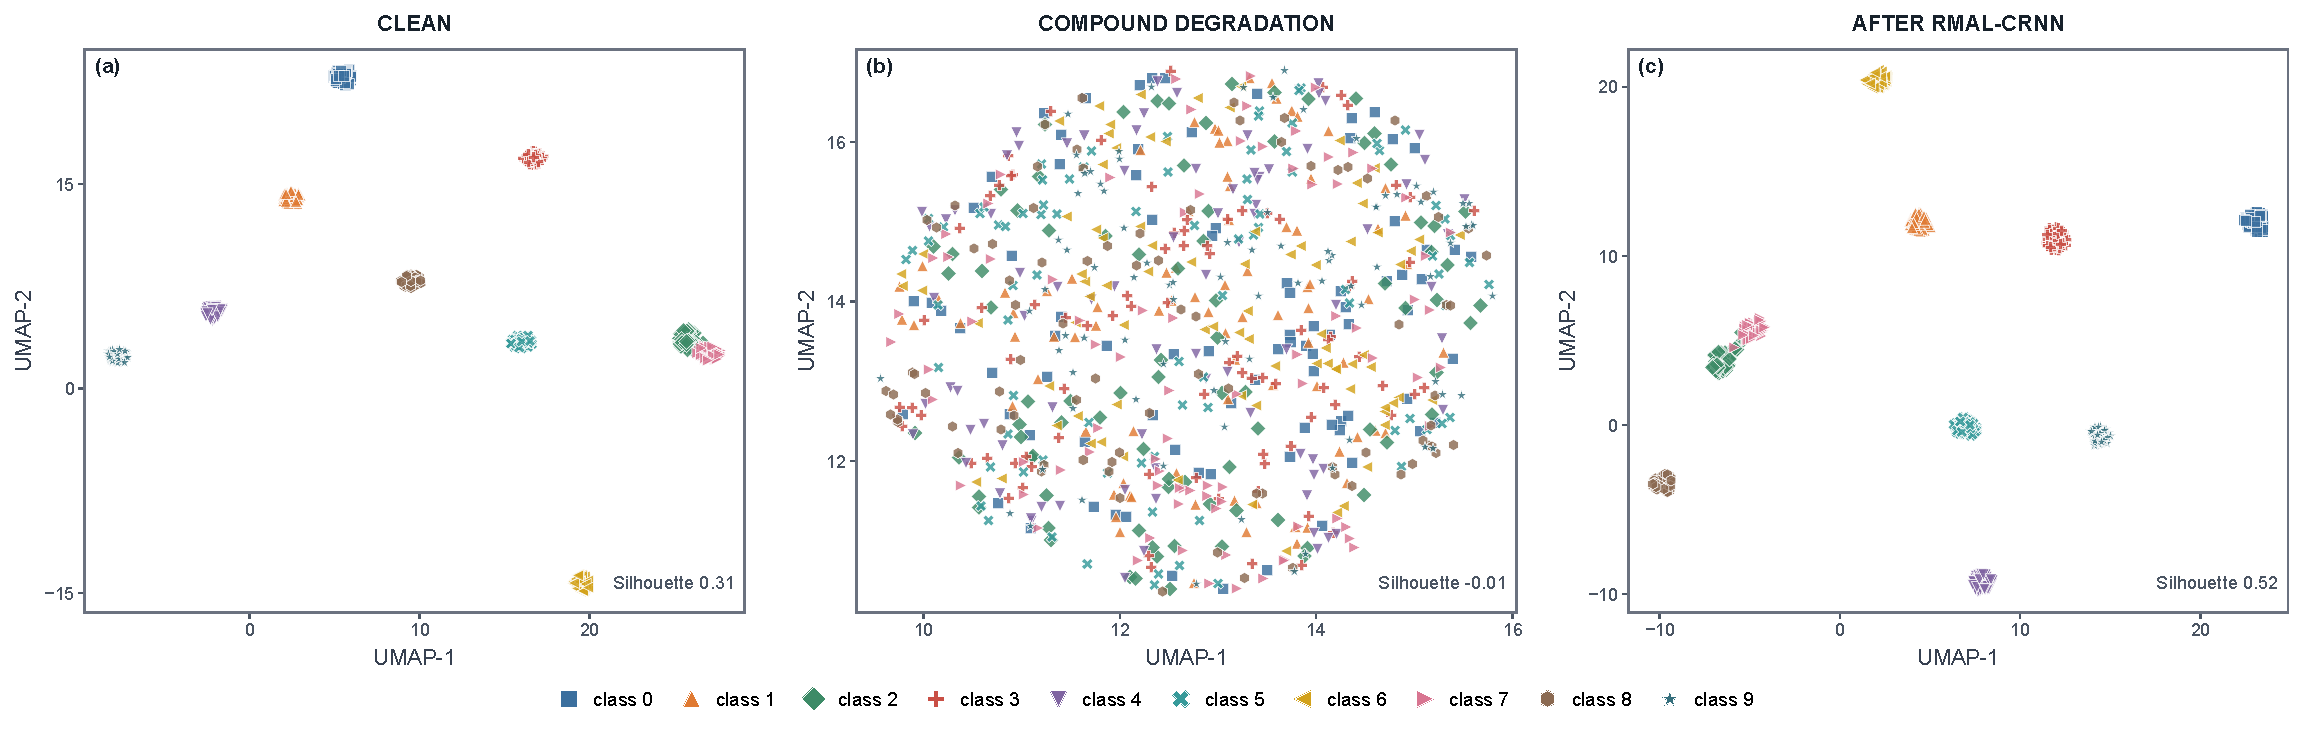
\includegraphics[width=\linewidth]{figures/fig3a.pdf}\\[0.72em]
  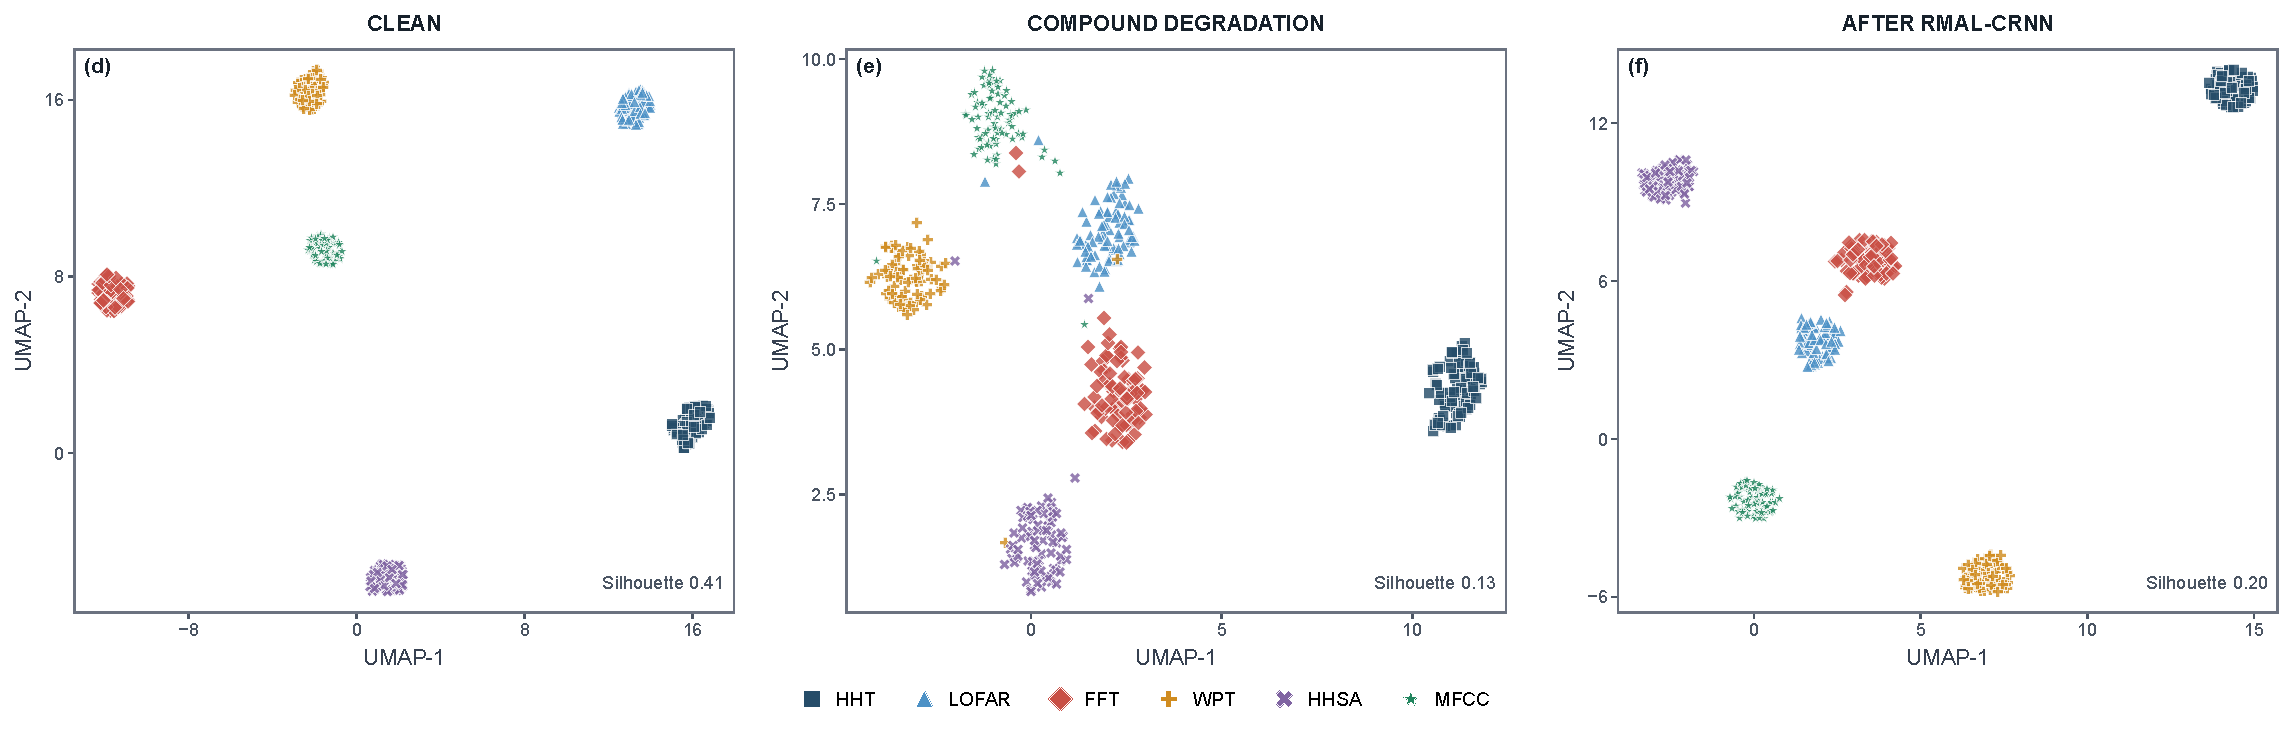
\includegraphics[width=\linewidth]{figures/fig3b.pdf}
  \caption{UMAP diagnostics under compound degradation. Top: clean, corrupted, and RMAL-CRNN sample embeddings. Bottom: clean, corrupted, and reliability-conditioned product-tangent descriptor embeddings.}
  \label{fig:compound-geometry}
\end{figure}

\subsection{Q2: Robust Classification}
Table~\ref{tab:comparison} compares sequence, convolutional, attention, forecasting, and manifold-oriented models on both benchmarks. RMAL-CRNN has the highest listed mean throughout. On Kielce it reaches $86.30\%$ and $93.88\%$ at $-5$ and $0$ dB, exceeding the strongest baseline by $2.27$ and $3.03$ points. On Glasgow it reaches $81.18\%$ at $0$ dB versus $74.28\%$ for CRNN, and remains ahead at lower SNRs. The consistent gains across both released benchmarks demonstrate the value of reliability-conditioned relation learning for low-SNR acoustic recognition.

\begin{table*}[t]
\caption{Accuracy across SNRs (\%, mean $\pm$ sample standard deviation) on the ten-class Kielce UAV-model benchmark (a) and the eight-class Glasgow/ACSAC~2022 acoustic-identity benchmark (b).}
\label{tab:comparison}
\centering
\small
\setlength{\tabcolsep}{2pt}
\textbf{(a) Kielce, ten classes}\par\vspace{0.25em}
\begin{tabular}{@{}lcccc@{}}
\toprule
Model (literature index) & $-5$ dB & $0$ dB & $5$ dB & $10$ dB\\
\midrule
MAtt-A \citep{pan2022matt} & $69.65{\pm}1.07$ & $80.33{\pm}1.43$ & $84.50{\pm}1.41$ & $88.65{\pm}1.17$\\
InceptionTime \citep{fawaz2020inceptiontime} & $78.90{\pm}0.79$ & $86.30{\pm}0.42$ & $90.75{\pm}0.70$ & $94.65{\pm}0.50$\\
CNN-Transformer \citep{vaswani2017attention} & $79.55{\pm}0.97$ & $86.83{\pm}0.48$ & $91.23{\pm}0.70$ & $93.85{\pm}0.45$\\
CRNN \citep{cakir2017crnn} & $80.80{\pm}0.82$ & $87.15{\pm}0.33$ & $91.80{\pm}0.34$ & $94.68{\pm}0.64$\\
SEResNet1D \citep{hu2020senet} & $81.98{\pm}0.49$ & $89.28{\pm}0.13$ & $92.73{\pm}0.52$ & $95.78{\pm}0.46$\\
TCN \citep{bai2018tcn} & $83.70{\pm}1.22$ & $90.85{\pm}0.49$ & $93.15{\pm}0.19$ & $96.28{\pm}0.39$\\
TimeMixer++ \citep{wang2025timemixerpp} & $84.03{\pm}1.21$ & $89.48{\pm}0.78$ & $93.68{\pm}0.60$ & $96.68{\pm}0.49$\\
MambaSL \citep{jung2026mambasl} & $82.53{\pm}1.15$ & $89.28{\pm}1.07$ & $93.20{\pm}0.18$ & $95.98{\pm}0.36$\\
RMAL-CRNN (ours) & \textbf{$86.30{\pm}0.29$} & \textbf{$93.88{\pm}0.36$} & \textbf{$96.08{\pm}0.35$} & \textbf{$97.48{\pm}0.51$}\\
\bottomrule
\end{tabular}
\par\vspace{0.65em}
\textbf{(b) Glasgow/ACSAC 2022 \citep{diao2022drone}, eight classes}\par\vspace{0.25em}
\begin{tabular}{@{}lcccc@{}}
\toprule
Model (literature index) & $-15$ dB & $-10$ dB & $-5$ dB & $0$ dB\\
\midrule
MAtt-A \citep{pan2022matt} & $30.35{\pm}1.38$ & $41.68{\pm}1.78$ & $54.43{\pm}1.23$ & $65.12{\pm}0.41$\\
InceptionTime \citep{fawaz2020inceptiontime} & $38.90{\pm}1.27$ & $54.25{\pm}1.51$ & $66.85{\pm}0.72$ & $75.02{\pm}1.31$\\
CNN-Transformer \citep{vaswani2017attention} & $38.32{\pm}0.34$ & $55.10{\pm}0.57$ & $69.12{\pm}0.66$ & $78.53{\pm}0.40$\\
CRNN \citep{cakir2017crnn} & $35.35{\pm}1.15$ & $51.38{\pm}1.02$ & $66.50{\pm}1.75$ & $74.28{\pm}0.62$\\
SEResNet1D \citep{hu2020senet} & $40.75{\pm}0.19$ & $56.12{\pm}0.88$ & $69.38{\pm}1.04$ & $78.50{\pm}1.13$\\
SPDNet \citep{huang2017spdnet} & $34.62{\pm}0.21$ & $46.03{\pm}1.45$ & $61.85{\pm}1.45$ & $70.88{\pm}2.43$\\
TCN \citep{bai2018tcn} & $36.35{\pm}1.31$ & $50.30{\pm}0.52$ & $65.05{\pm}1.50$ & $74.95{\pm}0.58$\\
BiLSTM \citep{graves2005bilstm} & $36.42{\pm}0.57$ & $50.68{\pm}1.84$ & $65.83{\pm}1.14$ & $73.95{\pm}0.44$\\
RMAL-CRNN (ours) & \textbf{$45.28{\pm}1.21$} & \textbf{$62.70{\pm}0.91$} & \textbf{$74.10{\pm}0.88$} & \textbf{$81.18{\pm}1.64$}\\
\bottomrule
\end{tabular}
\end{table*}

Figure~\ref{fig:confusion} complements the aggregate results with class-wise behavior at $0$ dB. In the reported run, HHT and HHSA exhibit broader off-diagonal errors, and direct concatenation does not recover the strongest individual-domain structure. RMAL-CRNN produces the most concentrated diagonal among the displayed matrices. This panel provides a class-wise view alongside the aggregate paired analysis below.

\begin{figure}[t]
  \centering
  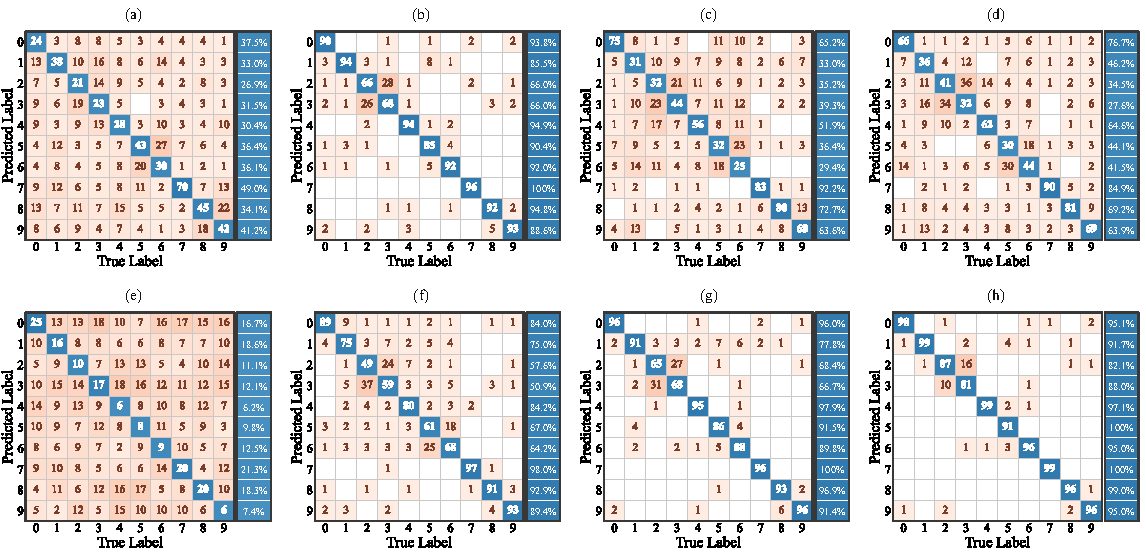
\includegraphics[width=0.98\linewidth]{figures/fig4.pdf}
  \caption{Confusion matrices at $0$ dB: (a) HHT, (b) LOFAR, (c) FFT, (d) WPT, (e) HHSA, (f) MFCC, (g) descriptor concatenation, and (h) RMAL-CRNN. Cell entries are counts; right-margin percentages are row-wise precision for each predicted class.}
  \label{fig:confusion}
\end{figure}

\subsection{Q3: Component Necessity}
We remove one operation at a time with fixed data and training settings. Exact full-model parameter counts, including the CRNN classifier, are given in Appendix~\ref{app:implementation}. Table~\ref{tab:ablation} reports losses of $1.41$, $1.50$, and $1.80$ points without FNSAR, LMA, and GST, and $6.96$ points against the CRNN control. Changes use unrounded paired run differences, explaining the apparent $0.01$ discrepancy from subtracting the rounded RMA-CRNN means. The ablation results use multiple random seeds, and the paired statistics summarize these runs.

The reported paired tests provide a second summary of the ablation runs: all listed $95\%$ confidence intervals for the complete-minus-control difference have positive lower bounds, and the reported Holm--Bonferroni-adjusted $p$-values are below $0.05$. Together with the component ablations, these results identify reliability estimation, tangent-metric relation learning, and sparse temporal affinity as complementary sources of the observed gain.

\begin{table}[t]
\caption{Structural ablations at $0$ dB (\%, mean $\pm$ standard deviation).}
\label{tab:ablation}
\centering
\small
\begin{tabular}{@{}llcc@{}}
\toprule
Variant & Composition & Accuracy & Change\\
\midrule
RMAL-CRNN & GST + LMA + FNSAR & $93.89{\pm}0.33$ & --\\
RMA-CRNN & GST + LMA & $92.47{\pm}0.49$ & $-1.41$\\
RL-CRNN & GST + FNSAR & $92.39{\pm}0.52$ & $-1.50$\\
MAL-CRNN & LMA + FNSAR & $92.09{\pm}0.38$ & $-1.80$\\
CRNN & baseline & $86.93{\pm}0.35$ & $-6.96$\\
\bottomrule
\end{tabular}
\end{table}


\section{Scope and Future Work}
This study establishes the value of reliability-conditioned geometric learning for six synchronized descriptors, two public UAV benchmarks, and controlled acoustic degradations. The next step is to extend this representation to learned front ends, broader platform and reverberation conditions, and asynchronous multimodal streams, while studying cross-dataset transfer and modality-specific corruption.

\section{Conclusion}
Compound degradation makes relation learning difficult because synchronized descriptors lose reliability at different rates. RMAL-CRNN addresses this structure through an ordered representation path: coordinate reliability estimation, descriptor-wise product-tangent projection, head-specific tangent-metric relation learning, and sparse temporal-affinity refinement. Controlled mechanism tests and two public-data benchmarks show that this design improves low-SNR recognition, while multi-seed ablations demonstrate complementary gains from its constituent modules. The central contribution is to make reliability part of geometric relation estimation itself, yielding a representation that captures cross-domain structure obscured by unequal descriptor quality.

Future work will extend this framework to heterogeneous multimodal inputs. Audio, vision, radio-frequency, and other sensing streams call for modality-specific reliability estimation, geometry-aware cross-modal alignment, and stable learning under missing or corrupted modalities. Broader cross-dataset evaluation, learned front ends, and efficient long-sequence affinity models will further develop its use in real-world acoustic and multimodal recognition.

\subsection*{Statements}
\textbf{AI use.} OpenAI Codex assisted with literature discovery and record checking, manuscript language editing, LaTeX preparation, equation-to-code checks, and the reviewer response. The authors are responsible for verifying the final manuscript, citations, code, and experimental results. \textbf{Ethics.} UAV acoustic recognition has safety and dual-use risks; deployment requires authorization, data governance, false-alarm assessment, and human oversight. \textbf{Reproducibility.} The appendices and code package provide the Zenodo source-data record, feature construction, selected training settings, model code, and mathematical details. Ablation results summarize multiple random seeds; the appendix specifies the retained experimental protocol and materials.

\bibliography{references}
\bibliographystyle{iclr2027_conference}

\appendix
\section{Experimental and Implementation Details}
\label{app:experimental-details}

\subsection{Frame and Descriptor Construction}
Let $r[n]$ be the real-valued sampled signal at discrete sample index $n$. The $t$-th length-$L$ frame with hop $\Delta$ is
\begin{equation}
\mathbf r_t=
\big[r[(t-1)\Delta],\ldots,r[(t-1)\Delta+L-1]\big]^\top.
\end{equation}
Each frame is transformed into HHT, LOFAR, FFT, WPT, HHSA, and MFCC blocks. The implementation standardizes each block to 32 coordinates and retains fixed block boundaries throughout training. The six synchronized blocks retain the identity of their respective descriptor domains while representing the same acoustic frame.

\subsection{Controlled Source and Degradation Model}
At continuous time $\tau$, the class-$c$ source $s_c(\tau)$ combines harmonic orders, modulated broadband fluctuations, and periodic ringing, consistent with measured multirotor modulation \citep{fang2022uav,gan2025modulation} and rotating-machine cyclostationarity \citep{antoni2009cyclostationarity}:
\begin{align}
s_c(\tau) &= \varpi_{\mathrm B}\sin(2\pi f_{\mathrm B}^{(c)}\tau)
 +\varpi_{2\mathrm B}\sin(4\pi f_{\mathrm B}^{(c)}\tau) \nonumber\\
&\quad +\varpi_{\mathrm w}w(\tau)
\bigl[1+\varpi_{\mathrm M}\sin(2\pi f_{\mathrm M}^{(c)}\tau)\bigr] \nonumber\\
&\quad +\varpi_{\mathrm r}\sin(2\pi f_{\mathrm b}\tau)
\exp[-\beta_0(\tau\bmod\tau_0)/a_{\mathrm R}^{(c)}].
\label{eq:source-signal-app}
\end{align}
Here $f_{\mathrm B}^{(c)}$ and $f_{\mathrm M}^{(c)}$ are the blade-passing and modulation rates, $a_{\mathrm R}^{(c)}$ is the class-dependent envelope divisor, and $\tau_0=1$ s; $f_{\mathrm b}$ is the ringing frequency; $w(\tau)$ is 1-kHz low-pass noise; and the $\varpi$ coefficients and $\beta_0$ control relative component strengths and ringing decay. The normalized controls are
$(\varpi_{\mathrm B},\varpi_{2\mathrm B},\varpi_{\mathrm w},\varpi_{\mathrm M},\varpi_{\mathrm r},\beta_0)=(1,0.5,0.4,0.8,0.8,30)$; classes differ through the two rates and envelope divisor. The envelope matches the supplied simulator expression \texttt{(t \% 1.0) / fr}, where \texttt{fr} stores $a_{\mathrm R}^{(c)}$.

After coherent delayed paths, a turbulence envelope, and Doppler phase, the three controlled additive degradations are applied to form $r_{\mathrm{sim}}(\tau)$:
\begin{align}
r_{\mathrm{sim}}(\tau)
&=\Re\!\left\{\operatorname{HT}\!\left[
\sum_{p=0}^{P}\chi_p s_c(\tau-\delta_p)
g_{\mathrm{turb}}(\tau)\right]e^{\mathrm i\Phi_{\mathrm{dop}}(\tau)}\right\}
\nonumber\\
&\quad+\varepsilon_{\mathrm{imp}}(\tau;\kappa)
+J(\tau;\mathrm{SIR})+v(\tau;\mathrm{SNR}).
\label{eq:degradation-app}
\end{align}
Here $P$ is the maximum path index, $\chi_p$ and $\delta_p$ are path gain and delay, the delays use circular shifts of the sampled source, $g_{\mathrm{turb}}$ is the turbulence envelope, $\Phi_{\mathrm{dop}}$ is Doppler phase, $\operatorname{HT}$ forms the analytic representation, and $\Re\{\cdot\}$ takes its real part. The terms $\varepsilon_{\mathrm{imp}}$, $J$, and $v$ denote sparse impulses, a competing source, and diffuse noise; $\kappa$, SIR, and SNR independently control their strengths. Their simultaneous application defines the compound condition. The turbulence envelope follows a low-pass random modulation motivated by physics-based acoustic scintillation models \citep{bresciani2023scintillation}.

\subsection{Public-Data Classes}
The ten-class Kielce subset is identified by the released class folders and UAV-model labels in Table~\ref{tab:kielce-models}. It contains five quadrotor (X4) and five hexarotor (X6) classes. The public collection is available at the \href{https://zenodo.org/records/15190811}{Zenodo record 15190811} \citep{miesikowska2023uavdataset}.

\begin{table}[t]
\caption{Ten UAV-model classes used from the Kielce acoustic dataset.}
\label{tab:kielce-models}
\centering
\scriptsize
\begin{tabular}{@{}cllll@{}}
\toprule
Structure & Class & UAV model & Date & Place\\
\midrule
X4 & D1 (\texttt{drone\_D1}) & MATRICE 300 & 15.03.2023 & Kielce\\
X4 & D2 (\texttt{drone\_D2}) & Mavic 3 & 15.03.2023 & Kielce\\
X4 & D3 (\texttt{drone\_D3}) & Mavic Air 2S & 15.04.2023 & Gdansk\\
X4 & D4 (\texttt{drone\_D4}) & Mavic Air 2 & 15.04.2023 & Gdansk\\
X4 & D10 (\texttt{drone\_D10}) & Mavic 2 Zoom & 17.04.2023 & Debogorze\\
X6 & D12 (\texttt{drone\_D12}) & Yuneec H520 & 17.04.2023 & Debogorze\\
X6 & D13 (\texttt{drone\_D13}) & Yuneec H520E RTK & 17.04.2023 & Debogorze\\
X6 & D14 (\texttt{drone\_D14}) & S900 & 18.04.2023 & Lapalice\\
X6 & D15 (\texttt{drone\_D15}) & X6D & 18.04.2023 & Lapalice\\
X6 & D16 (\texttt{drone\_D16}) & Y6 & 18.04.2023 & Lapalice\\
\bottomrule
\end{tabular}
\end{table}

\section{Additional Mechanism Diagnostics}
\label{app:mechanism-panels}

These panels expand the three diagnostics in Figure~\ref{fig:mechanisms}. Figure~\ref{fig:impulse-app} shows unequal descriptor sensitivity and selective GST correction, Figure~\ref{fig:cochannel-app} isolates the scale response of LMA against an unnormalized control, and Figure~\ref{fig:noise-app} reports the descriptor and temporal-compaction quantities used for FNSAR.

\begin{figure}[h]
  \centering
  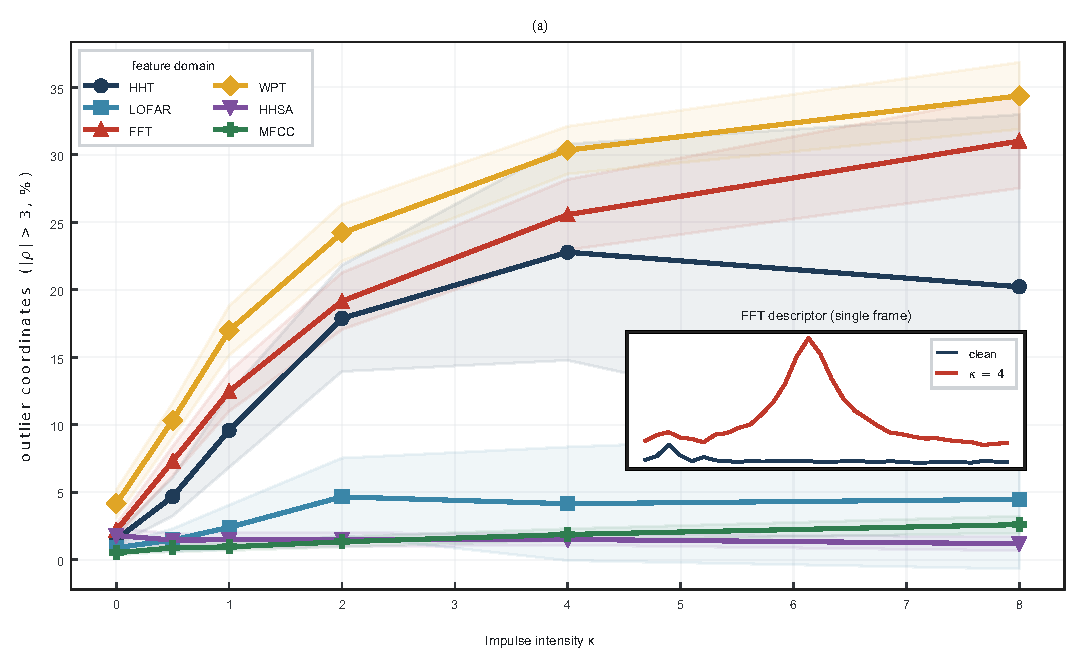
\includegraphics[width=\linewidth]{figures/fig5a.pdf}\\[-0.3em]
  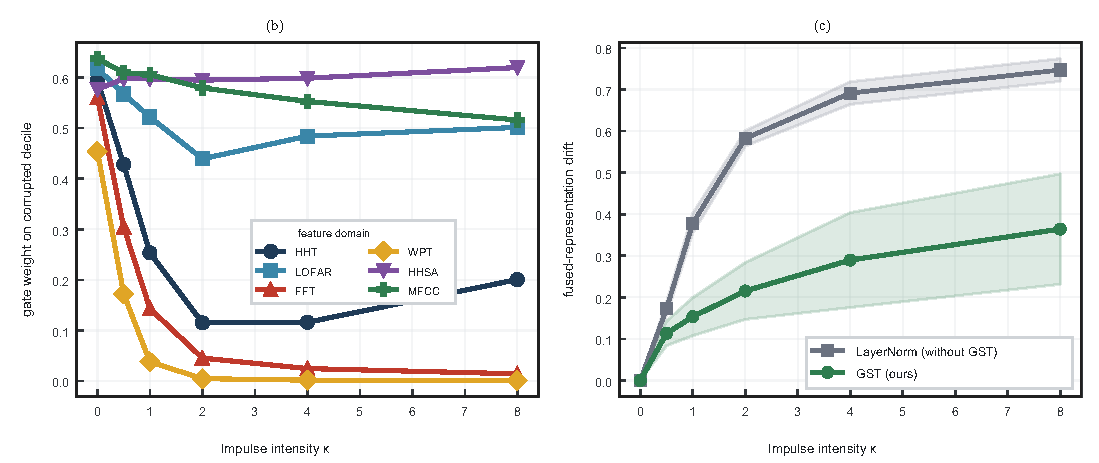
\includegraphics[width=\linewidth]{figures/fig5b.pdf}
  \caption{Impulsive corruption affects the six descriptor domains unequally. Learned reliability weights change selectively, and the corrected fused representation drifts more smoothly from its clean reference than the LayerNorm control in the evaluated range.}
  \label{fig:impulse-app}
\end{figure}

\begin{figure}[h]
  \centering
  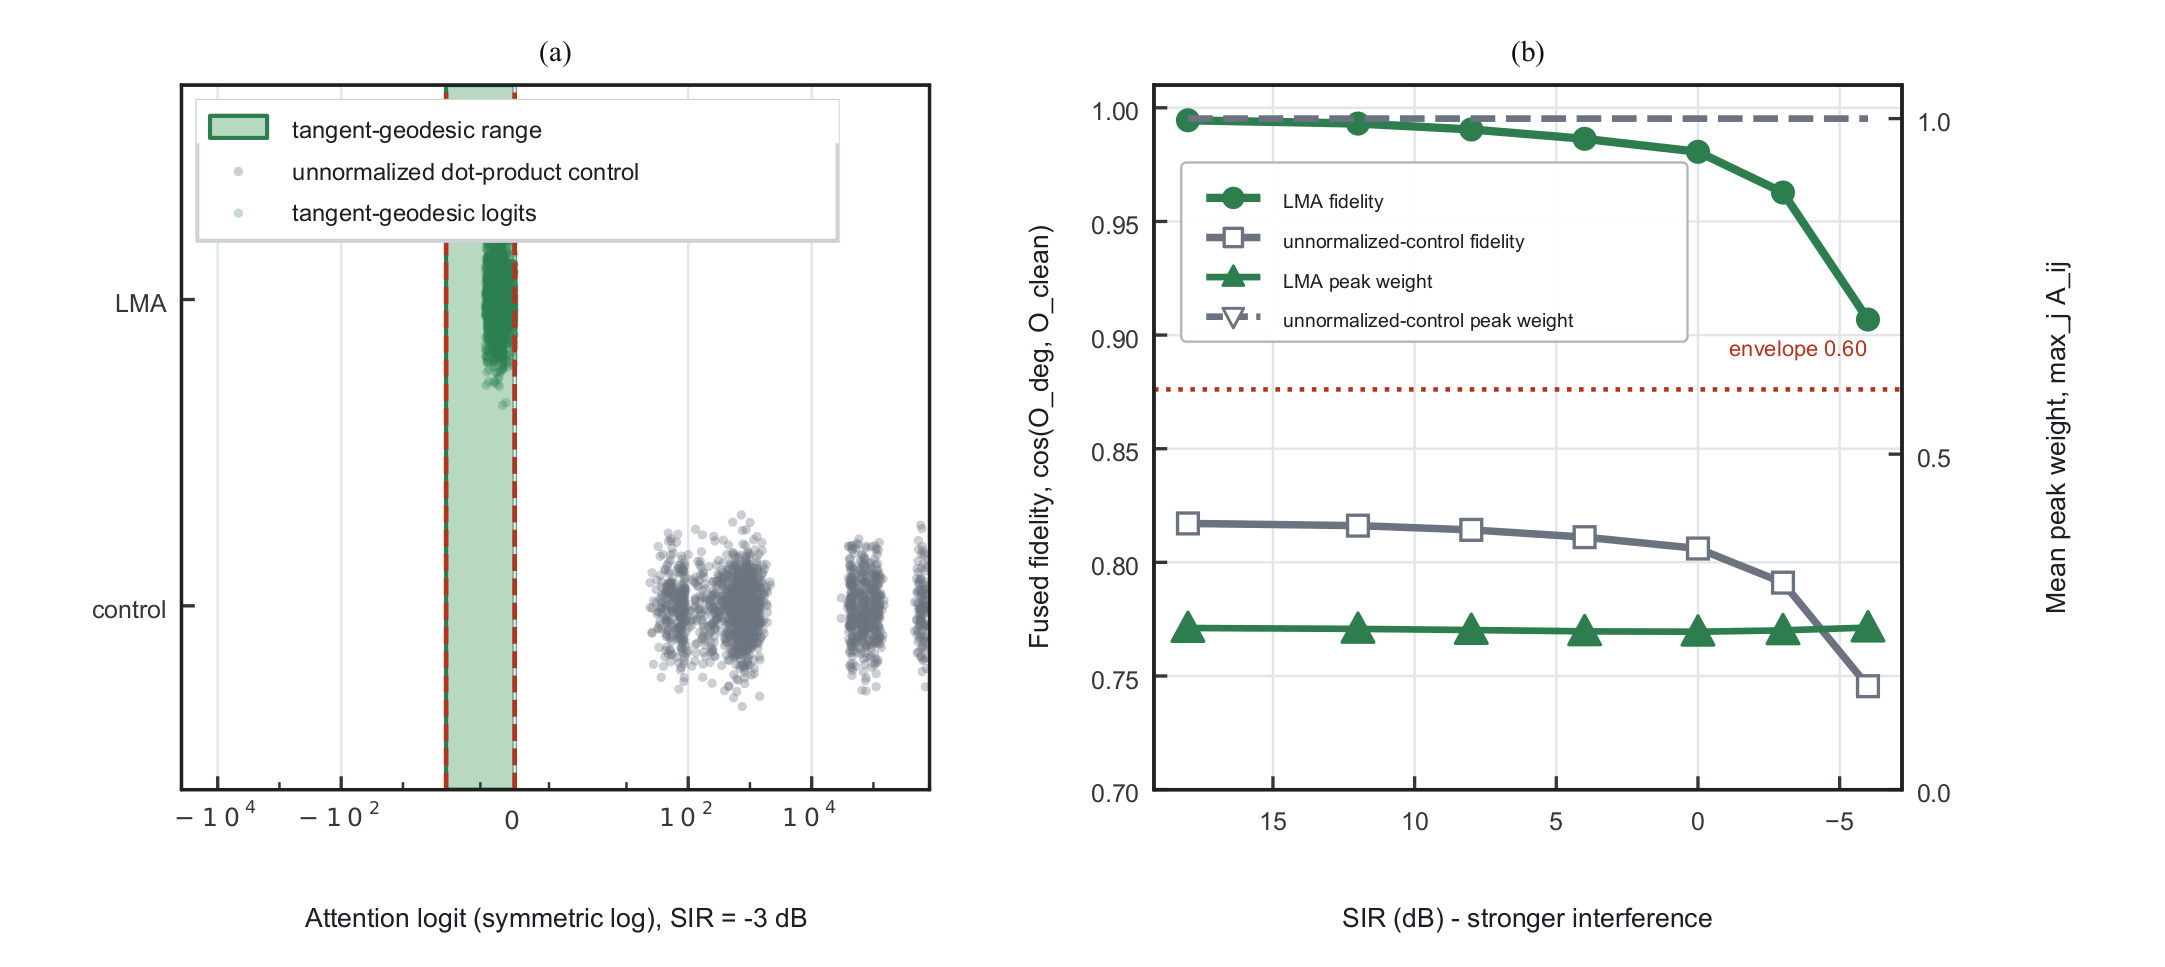
\includegraphics[width=\linewidth]{figures/fig6.png}
  \caption{Tangent-metric attention under co-channel interference. The diagnostic fixes $\gamma=0.50$; normalized projected logits stay within their admissible interval, whereas the unnormalized dot-product control is scale-sensitive.}
  \label{fig:cochannel-app}
\end{figure}

\begin{figure}[h]
  \centering
  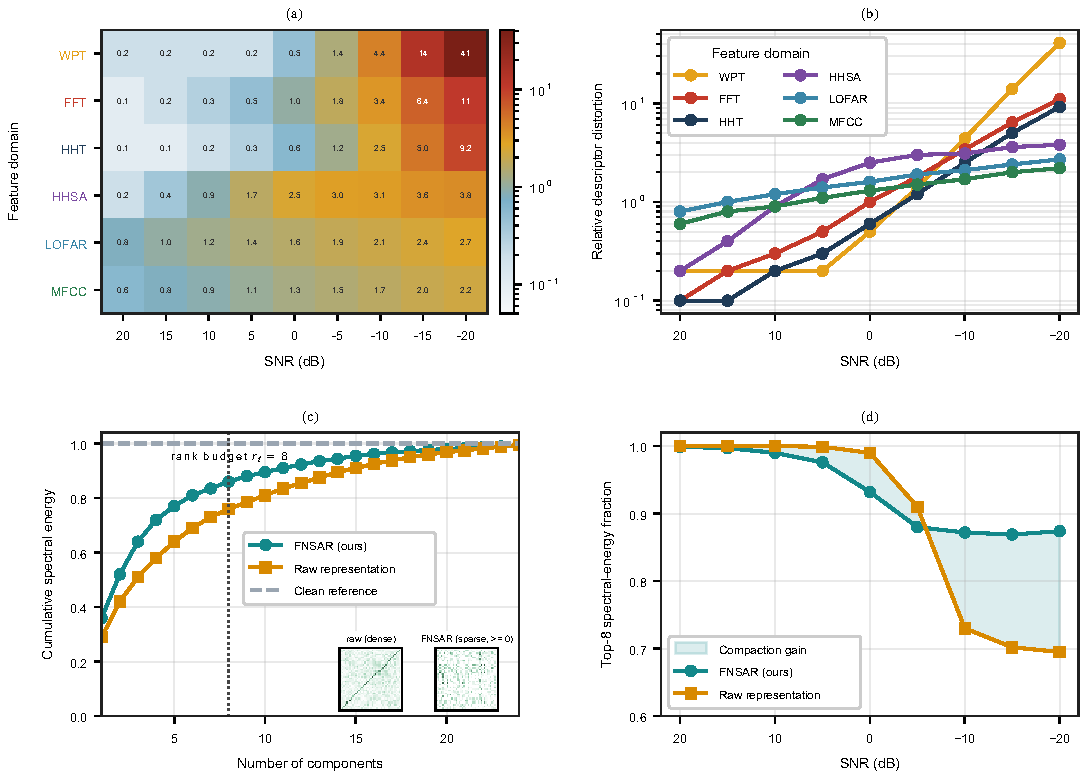
\includegraphics[width=0.94\linewidth]{figures/fig7.pdf}
  \caption{Descriptor sensitivity and factorized sparse temporal-affinity behavior under additive Gaussian noise.}
  \label{fig:noise-app}
\end{figure}

\section{Complete Paired Statistics}

\begin{table}[h]
\caption{Paired Student $t$-tests between RMAL-CRNN and control variants at $0$ dB over the paired multi-seed runs (Holm--Bonferroni corrected). Differences use unrounded paired runs.}
\label{tab:paired-test-app}
\centering
\small
\begin{tabular}{@{}lccccc@{}}
\toprule
Control & Difference & 95\% CI & $t$ & $d_z$ & Holm $p$\\
\midrule
RMA-CRNN & $+1.41$ & $[+0.77,+2.05]$ & $+5.41$ & $+2.05$ & $1.6\times10^{-3}$\\
RL-CRNN & $+1.50$ & $[+1.03,+1.97]$ & $+7.78$ & $+2.94$ & $7.1\times10^{-4}$\\
MAL-CRNN & $+1.80$ & $[+1.20,+2.40]$ & $+7.35$ & $+2.78$ & $7.1\times10^{-4}$\\
CRNN & $+6.96$ & $[+6.69,+7.22]$ & $+63.95$ & $+24.17$ & $3.9\times10^{-9}$\\
\bottomrule
\end{tabular}
\end{table}

\section{Implementation and Sensitivity}
\label{app:implementation}

The selected attention head count is $N_h=4$, factor rank $r_\ell=8$, and fusion dimension $d_f=64$. The learning rate is $10^{-3}$ and batch size is 32. These values come from the repeated scans summarized in Figure~\ref{fig:hyperparameters-app}; the scan characterizes sensitivity around the selected configuration.

All classification results use the benchmark-specific fixed splits and multiple random seeds. We report mean accuracy with sample standard deviation, and paired comparisons use matched runs. Training uses AdamW with learning rate $10^{-3}$ and weight decay $10^{-4}$, cosine learning-rate decay, batch size 32, label smoothing 0.1, gradient clipping at 2, and stochastic weight averaging over the final 30 of 120 epochs. The ablation configuration uses a stratified 60\%/20\%/20\% split with split seed 42.

The full-model parameter count was independently recounted by instantiating the retained PyTorch architecture. It includes the feature pipeline and the CNN--BiLSTM classifier; the parameter count of the proposed modules alone is not the total-model count.
\begin{table}[h]
\caption{Trainable parameter count for the retained ten-class implementation.}
\label{tab:parameter-breakdown}
\centering
\small
\begin{tabular}{@{}lr@{}}
\toprule
Component & Parameters\\
\midrule
GST gates and tangent embeddings & 960\\
LMA, including domain embeddings & 4,388\\
Fusion projection and FNSAR & 13,442\\
CNN--BiLSTM classifier & 320,586\\
\midrule
RMAL-CRNN total & 339,376\\
CRNN control total & 333,322\\
\bottomrule
\end{tabular}
\end{table}
These counts correspond to \texttt{RMALCRNN} and \texttt{BaselineCRNN} in \texttt{ablation.py}. The CRNN has two Conv1D--BatchNorm--ReLU--pool blocks (64/128 channels; kernels 7/3), one bidirectional LSTM (128 hidden units per direction), dropout 0.5, temporal mean pooling, and a linear classifier. The $192\times64$ fusion matrix receives QR initialization and is then trained freely. GST and LMA are implemented by \texttt{StudentTRobustGate}, \texttt{SphericalTangentEmbedding}, and \texttt{LogMapTangentAttention}; FNSAR is \texttt{DiffNSLLR}.

\begin{figure}[h]
  \centering
  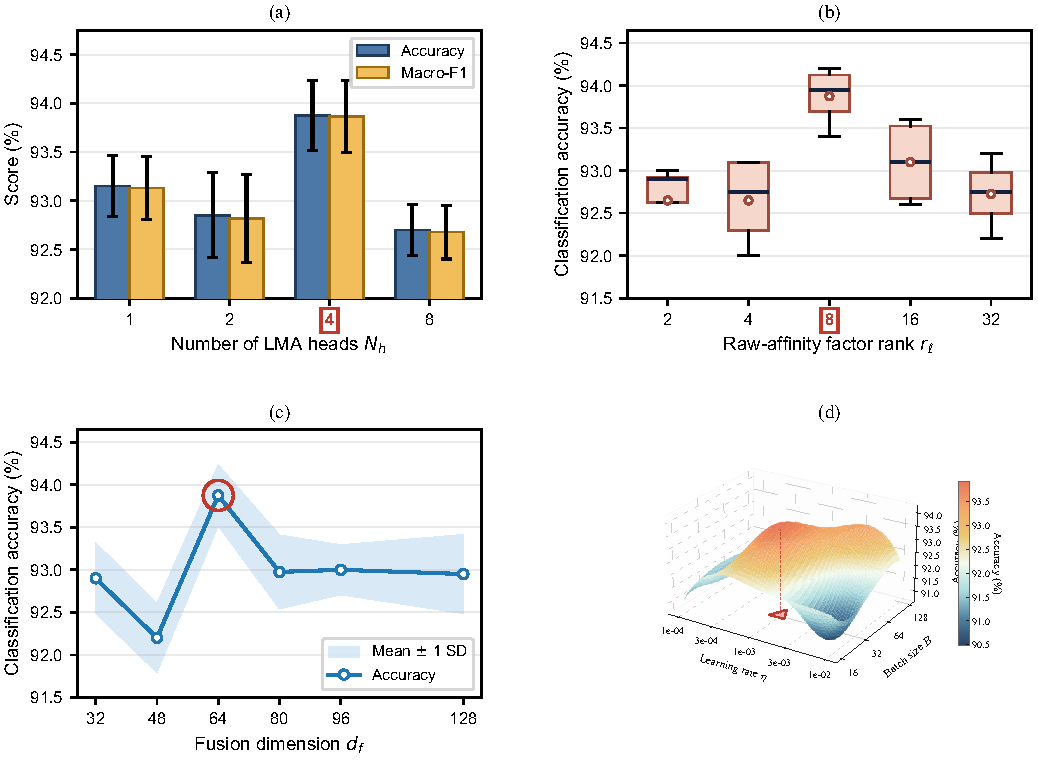
\includegraphics[width=\linewidth]{figures/fig8.pdf}
  \caption{Sensitivity to attention heads, factor rank, fusion dimension, and the learning-rate/batch-size pair.}
  \label{fig:hyperparameters-app}
\end{figure}

The architectures in \texttt{compare.py} are specified directly by their model classes. InceptionTime \citep{fawaz2020inceptiontime} has six Inception modules; CNN-Transformer has two strided Conv1D layers followed by a three-layer, eight-head encoder ($d=128$, feed-forward width 256); SEResNet1D has a convolutional stem and three squeeze-and-excitation residual blocks with channels $(64,128,128)$ \citep{hu2020senet}; TCN uses dilations $(1,2,4,8)$ \citep{bai2018tcn}. SPDNet uses BiMap/ReEig layers and a LogEig classifier \citep{huang2017spdnet}, and BiLSTM uses two bidirectional recurrent layers.

\paragraph{MAtt identity and acoustic adaptation.}
MAtt-A is the acoustic adaptation of the SPD manifold-attention architecture introduced by Pan, Chou, and Wei \citep{pan2022matt} (NeurIPS 2022), implemented as \texttt{MAtt} in \texttt{compare.py}. It has a $192\!\to\!40\!\to\!16$ Conv1D front end, four window-covariance tokens, QR-parameterized BiMap query/key/value maps, Log-Euclidean attention, and a LogEig/vectorization classifier. For SPD queries $\mathbf Q_i$, keys $\mathbf K_j$, and values $\mathbf V_j$, the implemented weights $a_{ij}$ and output $\mathbf O_i$ are
\begin{equation}
a_{ij}=\operatorname{softmax}_{j}\!\left[-|\tau|\sqrt{\|\log\mathbf Q_i-\log\mathbf K_j\|_F^2+10^{-8}}\right],
\qquad \mathbf O_i=\exp\!\left(\sum_j a_{ij}\log\mathbf V_j\right),
\label{eq:matt-adaptation}
\end{equation}
where $\tau$ is a learned scale and matrix log/exp use stabilized eigendecompositions. The acoustic adaptation uses covariance shrinkage 0.3 and diagonal loading $10^{-3}$. The original EEG formulation uses trace-normalized covariance and a different similarity transform, while ManifoldNet is a separate related method.

\paragraph{Additional comparison records.}
TimeMixer++ \citep{wang2025timemixerpp} and MambaSL \citep{jung2026mambasl} are included as sequence-classification baselines. Their formal publications are cited in Table~\ref{tab:comparison}; the MAtt-A acoustic adaptation is specified above.

TimeMixer++ Macro-F1 is $84.00{\pm}1.16$, $89.44{\pm}0.77$, $93.68{\pm}0.60$, and $96.67{\pm}0.49$ at $-5$, $0$, $5$, and $10$ dB. MambaSL Macro-F1 is $82.58{\pm}1.19$, $89.30{\pm}1.05$, $93.20{\pm}0.17$, and $95.97{\pm}0.36$. These results are reported as multi-seed means with sample standard deviations.

This appendix gives the proofs supporting the geometric interpretation and structural analysis in the main paper. It establishes a directional relation for the GST projection before normalization and bias, the concentration envelope of tangent-metric attention, and the factorized proximal structure of the temporal affinity.
\section{Blockwise Directional Equivalence on a Product of Spheres}
\label{app:blockwise}
\textbf{Proposition S.1:} Let \(K\geq1\) and \(d\geq2\). For every domain \(k\), assume \(\|\overline{\mathbf p}_k\|_2\geq\epsilon\) and let the gated vector in~\eqref{eq:domain-alignment} satisfy \(\mathbf h_t^{(k)}\neq\mathbf0\), and define
\label{prop:block-direction}
\begin{align}
\boldsymbol{\upsilon}_t^{(k)}
&=\frac{\mathbf h_t^{(k)}}{\|\mathbf h_t^{(k)}\|_2},
&\theta_{t,k}
&=\arccos\!\left((\boldsymbol{\upsilon}_t^{(k)})^\top\mathbf p_k\right),\nonumber\\
\mathbf u_t^{(k)}
&=\Pi_{\mathbf p_k}\mathbf h_t^{(k)},
&\omega_{t,k}
&=\frac{\theta_{t,k}}
{\|\mathbf h_t^{(k)}\|_2\sin\theta_{t,k}}.
\label{eq:app-block-definitions}
\end{align}
Assume \(\theta_{t,k}\in(0,\pi)\) for all \(k\). On the product manifold
\(\mathcal P=(\Sph^{d-1})^K\), stack the base points, normalized aligned vectors, and tangent components as \(\mathbf p=(\mathbf p_1,\ldots,\mathbf p_K)\), \(\boldsymbol{\upsilon}_t=(\boldsymbol{\upsilon}_t^{(1)},\ldots,\boldsymbol{\upsilon}_t^{(K)})\), and \(\mathbf u_t=[(\mathbf u_t^{(1)})^\top,\ldots,(\mathbf u_t^{(K)})^\top]^\top\in\R^{Kd}\). Then
\begin{equation}
\operatorname{Log}_{\mathbf p}(\boldsymbol{\upsilon}_t)
=\boldsymbol{\Omega}_t\mathbf u_t,
\qquad
\boldsymbol{\Omega}_t
=\operatorname{blkdiag}_{k=1}^{K}(\omega_{t,k}\mathbf I_d)\succ\mathbf0.
\label{eq:app-log}
\end{equation}
Hence each pre-normalization projected block is collinear with, and points in the same direction as, the corresponding spherical logarithmic map. The result characterizes the projected direction. With the implemented bias, \(\mathbf z_t^{(k)}-\mathbf b_k\in\Tangent_{\mathbf p_k}\Sph^{d-1}\), so the final token lies in the corresponding affine tangent space.

\emph{Proof:} The product-manifold logarithmic map is the concatenation of its component maps. For domain \(k\), the logarithmic map on \(\Sph^{d-1}\) is
\begin{equation}
\log_{\mathbf p_k}(\boldsymbol{\upsilon}_t^{(k)})
=\frac{\theta_{t,k}}{\sin\theta_{t,k}}
\left(\boldsymbol{\upsilon}_t^{(k)}
-\cos\theta_{t,k}\,\mathbf p_k\right).
\label{eq:app-log-map}
\end{equation}
Because
\(\cos\theta_{t,k}=(\mathbf h_t^{(k)})^\top\mathbf p_k/
\|\mathbf h_t^{(k)}\|_2\),
\begin{equation}
\boldsymbol{\upsilon}_t^{(k)}
-\cos\theta_{t,k}\,\mathbf p_k
=\frac{\Pi_{\mathbf p_k}\mathbf h_t^{(k)}}
{\|\mathbf h_t^{(k)}\|_2}
=\frac{\mathbf u_t^{(k)}}{\|\mathbf h_t^{(k)}\|_2}.
\label{eq:app-tangent}
\end{equation}
Substitution into~\eqref{eq:app-log-map} gives
\(\log_{\mathbf p_k}(\boldsymbol{\upsilon}_t^{(k)})
=\omega_{t,k}\mathbf u_t^{(k)}\). Stacking the \(K\) identities yields~\eqref{eq:app-log}. Since every \(\omega_{t,k}>0\), the direction of each nonzero block is preserved. At \(\theta_{t,k}=0\), both component vectors vanish and no direction is defined; at \(\theta_{t,k}=\pi\), the component logarithmic map is not unique.

The directional agreement follows because both constructions use the same orthogonal component \(\Pi_{\mathbf p_k}\mathbf h_t^{(k)}\), and spherical curvature multiplies it by a positive blockwise scale. Normalization preserves the direction of each nonzero component and controls its norm by \(\sqrt d\). The learned bias then translates the tangent representation, as specified in~\eqref{eq:token}.

\section{Concentration Analysis of Tangent-Metric Attention}
\label{app:attention-proof}
\textbf{Proposition S.2:} For head \(h\), let \(\|\mathbf p_h\|_2\leq1\) as ensured by the implemented normalization, and define
\label{prop:attention-concentration}
\begin{equation}
D_{\max}^{h}
=\max_{1\leq i,j\leq K}\|\mathbf q_i^h-\mathbf k_j^h\|_2^2
\leq4.
\label{eq:app-diameter}
\end{equation}
Then the logits and weights in~\eqref{eq:attention-logit}--\eqref{eq:attention-weight} satisfy
\begin{align}
-\gamma_hD_{\max}^{h}
&\leq \ell_{ij}^{h}\leq0,
\label{eq:app-logit-bound}\\
\max_j a_{ij}^{h}
&\leq\frac{1}{1+(K-1)e^{-\gamma_hD_{\max}^{h}}},
\label{eq:app-weight-bound}\\
\mathsf H(\mathbf a_{i,\cdot}^{h})
&\geq\log\!\left(
1+(K-1)e^{-\gamma_hD_{\max}^{h}}
\right).
\label{eq:app-entropy-bound}
\end{align}

\emph{Proof:} By~\eqref{eq:qkv},
\(\|\bar{\mathbf q}_i^h\|_2\leq1\) and
\(\|\bar{\mathbf k}_j^h\|_2\leq1\). The operator \(\mathbf I-\mathbf p_h\mathbf p_h^\top\) has spectral norm at most one for \(\|\mathbf p_h\|_2\leq1\), so
\(\|\mathbf q_i^h\|_2\leq1\) and
\(\|\mathbf k_j^h\|_2\leq1\). The triangle inequality gives
\(\|\mathbf q_i^h-\mathbf k_j^h\|_2\leq2\), proving~\eqref{eq:app-diameter};~\eqref{eq:app-logit-bound} then follows from \(\gamma_h>0\).

Let \(j^\star=\argmax_j \ell_{ij}^{h}\). The softmax can be written as
\begin{equation}
\max_j a_{ij}^{h}
=\frac{1}{1+
\sum_{m\neq j^\star}
e^{\ell_{im}^{h}-\ell_{ij^\star}^{h}}}.
\label{eq:app-softmax}
\end{equation}
The logit interval implies
\(\ell_{im}^{h}-\ell_{ij^\star}^{h}\geq-\gamma_hD_{\max}^{h}\). Lower-bounding every term in the denominator proves~\eqref{eq:app-weight-bound}. Finally, for any discrete distribution \(\mathbf a\),
\(\mathsf H(\mathbf a)\geq-\log\max_j a_j\), which gives~\eqref{eq:app-entropy-bound}.

For finite \(\gamma_h\) and \(K>1\), the peak-weight bound is strictly below one and the entropy bound is positive. The proposition therefore gives an explicit concentration envelope for tangent-metric attention at a finite inverse bandwidth. On the unit-normalization branch, the head-specific operator is a rank-\((d_h-1)\) orthogonal projector, selecting complementary tangent directions for cross-domain relations.

\section{Raw-Affinity Rank Budget, Proximal Sparsity, and Residual-Output Bound}
\label{app:affinity}
Let \(\mathbf F\in\R^{T\times d_f}\),
\(\mathbf W_u,\mathbf W_v\in\R^{r_\ell\times d_f}\), and define
\begin{alignat}{2}
\mathbf U
&=\mathbf F\mathbf W_u^\top
&\qquad&\in\R^{T\times r_\ell},
\label{eq:app-u}\\
\mathbf V
&=\mathbf F\mathbf W_v^\top
&&\in\R^{T\times r_\ell},
\label{eq:app-v}\\
\mathbf C_{\mathrm{raw}}
&=\frac{1}{\sqrt{r_\ell}}\mathbf U\mathbf V^\top
&&\in\R^{T\times T},
\label{eq:app-craw}\\
\mathbf C
&=\ReLU\!\left(
\mathbf C_{\mathrm{raw}}-\vartheta\mathbf1_T\mathbf1_T^\top
\right)
&&\in\R^{T\times T}.
\label{eq:app-c}
\end{alignat}

\textbf{Proposition S.3.1:} The pre-threshold affinity satisfies
\begin{equation}
\rank(\mathbf C_{\mathrm{raw}})\leq r_\ell,
\label{eq:app-rank}
\end{equation}
independent of \(T\).

\emph{Proof:} Since \(\mathbf U,\mathbf V\in\R^{T\times r_\ell}\),
\begin{equation*}
\rank(\mathbf U\mathbf V^\top)
\leq\min\{\rank(\mathbf U),\rank(\mathbf V)\}
\leq r_\ell.
\end{equation*}
Multiplication by \(1/\sqrt{r_\ell}\) preserves rank, and the bound is attained when both factors have full column rank. The elementwise threshold in~\eqref{eq:app-c} can increase matrix rank, so Proposition~S.3.1 applies only to the raw affinity. The proposition characterizes the compact pre-threshold relation, while Propositions~S.3.2--S.3.3 characterize the nonnegative sparse support and residual aggregation used by the network. Asymmetric entries encode directional temporal dependence, and diagonal entries retain frame self-information.

\textbf{Proposition S.3.2:} Let
\(g_{\vartheta}(\mathbf G)=\vartheta\|\mathbf G\|_1+\iota_{\geq0}(\mathbf G)\), where \(\|\cdot\|_1\) sums entrywise absolute values and \(\iota_{\geq0}\) is zero on the nonnegative orthant and \(+\infty\) elsewhere. Then
\begin{align}
\mathbf C
&=\argmin_{\mathbf G\geq0}
\frac{1}{2}\|\mathbf G-\mathbf C_{\mathrm{raw}}\|_F^2
+\vartheta\|\mathbf G\|_1,
\label{eq:app-prox-problem}\\
\mathbf C&=\prox_{g_{\vartheta}}(\mathbf C_{\mathrm{raw}}),
\label{eq:app-prox}
\end{align}
at fixed \(\mathbf C_{\mathrm{raw}}\), with
\begin{equation}
\vartheta_2>\vartheta_1
\ \Longrightarrow\
\operatorname{supp}(\mathbf C_{\vartheta_2})
\subseteq\operatorname{supp}(\mathbf C_{\vartheta_1}).
\label{eq:app-support}
\end{equation}

\emph{Proof:} The objective is separable. For one entry \(x=C_{\mathrm{raw},ts}\), solve
\begin{equation*}
\min_{g\geq0}\ \frac12(g-x)^2+\vartheta g.
\end{equation*}
Strict convexity gives the unique solution
\(g^\star=\max\{x-\vartheta,0\}\). Applying this result entry-wise proves~\eqref{eq:app-prox-problem}--\eqref{eq:app-prox}. Since \(C_{ts}>0\) exactly when \(C_{\mathrm{raw},ts}>\vartheta\), increasing \(\vartheta\) can only remove support.

\textbf{Proposition S.3.3:} Let the aggregated column vector be
\(\mathbf m_t=(\mathbf C\mathbf F)_{t,:}^{\top}
=\sum_{s=1}^{T}C_{ts}\mathbf f_s\) and
\begin{equation*}
\LN(\mathbf m_t)
=\boldsymbol{\psi}_{\mathrm{LN}}\odot\hat{\mathbf m}_t
+\mathbf b_{\mathrm{LN}},
\qquad
\|\hat{\mathbf m}_t\|_2\leq\sqrt{d_f}.
\end{equation*}
Here \(\hat{\mathbf m}_t\) is the centered, variance-normalized vector, and \(\boldsymbol\psi_{\mathrm{LN}}\) and \(\mathbf b_{\mathrm{LN}}\) are the learned gain and bias. For finite LayerNorm parameters, define
\begin{equation*}
G_{\mathrm{LN}}
=\|\boldsymbol{\psi}_{\mathrm{LN}}\|_\infty\sqrt{d_f}
+\|\mathbf b_{\mathrm{LN}}\|_2.
\end{equation*}
Then the output in~\eqref{eq:fnsar-output} satisfies
\begin{equation}
\|\mathbf f_t^{\mathrm{out}}\|_2
\leq(1-\zeta)\|\mathbf f_t\|_2+\zeta G_{\mathrm{LN}},
\label{eq:app-norm-bound}
\end{equation}
independent of the scale of \(\mathbf C\).

\emph{Proof:} The LayerNorm bound follows from
\begin{equation*}
\|\LN(\mathbf m_t)\|_2
\leq\|\boldsymbol{\psi}_{\mathrm{LN}}\|_\infty
\|\hat{\mathbf m}_t\|_2+\|\mathbf b_{\mathrm{LN}}\|_2
\leq G_{\mathrm{LN}}.
\end{equation*}
Applying the triangle inequality to~\eqref{eq:fnsar-output} gives
\begin{equation*}
\|\mathbf f_t^{\mathrm{out}}\|_2
\leq(1-\zeta)\|\mathbf f_t\|_2
+\zeta\|\LN(\mathbf m_t)\|_2,
\end{equation*}
and~\eqref{eq:app-norm-bound} follows. This establishes the LayerNorm-residual bound used by the temporal refinement.


\end{document}
